\documentclass[a4paper, english, 10pt]{report}


%% Language and font encodings
\usepackage[english]{babel}
\usepackage[utf8x]{inputenc}
\usepackage[T1]{fontenc}

%% Sets page size and margins
\usepackage[a4paper,top=2cm,bottom=2.5cm,left=2.5cm,right=2cm,marginparwidth=1cm]{geometry}

%% Useful packages
\usepackage{amsmath}
\usepackage{graphicx}
\usepackage[colorinlistoftodos]{todonotes}
\usepackage[colorlinks=true, allcolors=black]{hyperref}

%% Own packages
\usepackage{subfiles}
\usepackage{fancyhdr}
\usepackage{fancyref}
\usepackage{listings}
\usepackage{subcaption}
\usepackage[toc,page]{appendix}
\usepackage{natbib}

\setlength{\headheight}{30pt}
\bibliographystyle{plain}
\newcommand\NEVERRUNME{
    \bibliography{References.bib}
}

% Definings for inputcode in lisings
\usepackage{color}

\definecolor{mygreen}{rgb}{0,0.6,0}
\definecolor{mygray}{rgb}{0.5,0.5,0.5}
\definecolor{mymauve}{rgb}{0.58,0,0.82}
\definecolor{mypink}{rgb}{0,0.25,0.2}

\lstset{ %
	belowskip = 0pt,
  language = matlab,
  backgroundcolor=\color{white},   % choose the background color; you must add \usepackage{color} or \usepackage{xcolor}; should come as last argument
  basicstyle=\footnotesize,        % the size of the fonts that are used for the code
  breakatwhitespace=false,         % sets if automatic breaks should only happen at whitespace
  breaklines=true,                 % sets automatic line breaking
  captionpos=b,                    % sets the caption-position to bottom
  commentstyle=\color{mygreen},    % comment style
  deletekeywords={...},            % if you want to delete keywords from the given language
  escapeinside={\%*}{*)},          % if you want to add LaTeX within your code
  extendedchars=true,              % lets you use non-ASCII characters; for 8-bits encodings only, does not work with UTF-8
  frame=single,	                   % adds a frame around the code
  keepspaces=true,                 % keeps spaces in text, useful for keeping indentation of code (possibly needs columns=flexible)
  keywordstyle=\color{blue},       % keyword style
  morekeywords={pcl,PointCloud,::,Ptr,PointCloud2,line_t,line_p,lineRow_t,lineRow_p,landingField_p,landingField_t,PointXYZ},            % if you want to add more keywords to the set
  numbers=left,                    % where to put the line-numbers; possible values are (none, left, right)
  numbersep=5pt,                   % how far the line-numbers are from the code
  numberstyle=\tiny\color{mygray}, % the style that is used for the line-numbers
  rulecolor=\color{black},         % if not set, the frame-color may be changed on line-breaks within not-black text (e.g. comments (green here))
  showspaces=false,                % show spaces everywhere adding particular underscores; it overrides 'showstringspaces'
  showstringspaces=false,          % underline spaces within strings only
  showtabs=false,                  % show tabs within strings adding particular underscores
  stepnumber=2,                    % the step between two line-numbers. If it's 1, each line will be numbered
  stringstyle=\color{mymauve},     % string literal style
  tabsize=2,	                   % sets default tabsize to 2 spaces
  title=\lstname                   % show the filename of files included with \lstinputlisting; also try caption instead of title
}

% Fuss und Kopfzeile neu Definieren
\fancypagestyle{plain}{%
\fancyhf{} %alle Kopf- und Fußzeilenfelder bereinigen
\fancyfoot[R]{\thepage} %Seitennummer
%\fancyfoot[EL]{\thepage}
\fancyhead[L]{Bachelor Thesis}
\fancyhead[R]{Michael Kurmann}}

\pagestyle{plain}



% Title Page
\title{BAT - Sensor Fusion}
\author{Michael Kurmann}


\begin{document}
\begin{titlepage}
	\hbox{
			\hspace*{0.15\textwidth}
			\rule{1pt}{\textheight}
			\hspace*{0.05\textwidth}
			\parbox[b]{0.75\textwidth}{
{\scshape \large Lucerne University of Applied Science \& Architecture\par}
\vspace{0.2cm}
{\Huge \scshape \bfseries ARIS - Data Fusion for a Sounding Rocket\par}
\vspace{0.2cm}
{\scshape \large Bachelor Thesis\par}
\vspace{0.5cm}
\begin{center}
 
\includegraphics[height = 10cm]{Pictures/ARIS_TELL_Badge.png}
\end{center}



%\vspace{0.5cm}
\begin{flushleft}
\begin{tabular}{l l}

Author: & Michael Kurmann \\

Supervisor: & Prof. Marcel Joss\\

Expert: & Werner Scheidegger\\

Industrial Partner: & ARIS (Akademische Raumfahrt Initiative Schweiz) \\
		    & Oliver Kirchhoff\\

Submission date: & June 8, 2018\\
Classification: & Access
\end{tabular}
\end{flushleft}
\vspace{3cm}

}}

\vfill
\end{titlepage}


\chapter*{Declaration}
\thispagestyle{empty}
Hereby, I declare that I have composed the presented paper independently on my own and without any other resources than the ones indicated. All thoughts
taken directly or indirectly from sources are properly denoted as such.
This paper has neither been previously submitted to another authority nor has it been published yet.

\vspace{2cm}
Horw, \today

\begin{abstract}
\documentclass[main.tex]{subfiles} 

\begin{document}
That is the Abstract
\end{document}

\end{abstract}
\tableofcontents

\chapter{Introduction}
\label{ch:Introduction}

%\section{Tipps/Notes}
%  Pictures for what:
%  Aris logo ? 
%  Atmospheric model ? 
%  Different sensors ? 
%  Sensor Network
%  
%  
%  Problems found so far:
%  \begin{itemize}
%   \item How to calculate Height out of Pressure/Temp/Humidity Fabian version: $44330 * (1 - (\frac{pressure}{101325})^{ \frac{1}{5.255}})$
%   \item How to parameterize the different sensors (Measuring, Test Flight, Data Sheet ) ? 
%   \item How to fuse together Data from Sensors that have different Taus, especially those who are slower than the Loop-Time ?
%   \item How to integrate AirBreaks/Drag Force of Air/ Trust of Motor a input value?
%   \item What are the different noise factors and when do they occur ?
%   \item The up-flight is rather short: about 25 seconds, so the Fusion should have a small settling time
%   \item The Micro-Chip on which it is used is no the fastest : 168 MHz clock
%   \item The Ram on the Chip is not endless: Maximal space for the Sensor fusion is about 10kB
%   \item The Sensor Fusion should be as modular as possible so that it also can be used in the next competition
%   \item The Sensor Fusion has to be as sturdy as possible so that it will not fail if a problem occurs
%   \item The Fusion should make a state Estimation as precise as possible.
%   \item There are a lot of different variables: 3 Positions, 1 Speed, 3 Accelerations, 3 Lagen, Time, Pressure, Tempterature, Humidity, Up-/Downforce.
%   \item Especially the Input Value u which is the force onto the rocket is difficult to define (Drag, Trust = acceloration depends on wheigt which changes over time).
%   \item The different Sensor have different weaknesses: \begin{itemize}
% 							 \item Accelerometer: Offset, drift, weak to vibrations
%                                                          \item Gyro: Weak to Vibrations
%                                                          \item Barometer: Many uncertenties, unpercise
%                                                          \item GPS: Slow (max 5Hz)
%                                                         \end{itemize}
%                                                         
% 								  
%  \end{itemize}
 \section{Task}
 
 \begin{figure}[h!]
 \centering
 
\includegraphics[width=0.3\textwidth]{./Pictures/ARIS_TELL_Badge.png}
 % ARIS_TELL_Badge.png: 0x0 pixel, 300dpi, 0.00x0.00 cm, bb=
 \caption{Official logo of the competition project 2018}
 \label{fig:ArisTell}
\end{figure}

 The Academic Space Initiative Switzerland (ARIS) figure \ref{fig:ArisTell} is a student group which competes in the yearly Intercollegiate Rocket Engineering Competition (IREC).
 The goal of this competition is to build a rocket which can fly autonomous at a predefined apogee (10000 feet = 3048 meter) and after that return safe to the ground.
 There are a total of 1000 points to achieve in the competition which are split into different parts.
 
\begin{table}[h]
\centering
\begin{tabular}{|l|l|l|}\hline
{\bf Description} & {\bf Points} & {\bf Percent}\\\hline
Entry form an progress update & 60 & 6 \% \\ \hline
Technical report & 200 & 20 \% \\ \hline
Design implementation & 240 & 24 \% \\ \hline
Flight performance & 500 & 50 \% \\ \hline
Total & 1000 & 100 \% \\ \hline 
\end{tabular}
\caption{Calculation of the points of the IREC}
\label{tab:CompetitionCalculation}
\end{table}  

 Table \ref{tab:CompetitionCalculation} shows how those points are divided in detail. 
 It can be seen that just the halve of the points are assigned for the performance at the competition itself.
 The other halve of the points can be achieved by teamwork, professional documentation and engineering during the developing and construction of the rocket.
 For the 500 points which are assigned for the flight performance, 350 are assigned for the error made between the targeted and approached apogee.
 These points are calculated like this:
 
 $$ Points =  350 - \frac{350}{0.3\cdot TargetApogee} \cdot |TargetApogee - ActualApogee|$$
 
 So there is a total of one point loss per 2.6 meter error \cite{SpaceportAmericaCup2018}. \\
 To aim for the right apogee a Control algorithm is implemented.
 This algorithm relays on the information of different sensors to determine the rockets actual state.
 Because there are different sensors to measure the same value a algorithm which fuses those data would come in handy.
 With this fusion algorithm it should also be possible to be more accurate as with each sensor on its own.
 So the aim of this thesis is to implement a simulation and with its help find the algorithm which is most suitable for this task.\\
 For this the problem as well as the desired solution will be defined in this chapter.
 After that the models for the different sensor that will be used as well as the pro and con of different state estimators are discussed at beginning of chapter \ref{ch:Approach}.
 In addition, different possible system models are also described in this chapter.
 Chapter \ref{ch:Implementation} will then show, how the simulation and the fusion algorithm are implemented in detail.
 To verify that the implementation is working as intended, the results of the simulation are discussed in chapter \ref{ch:Tests}.
 In the last chapter \ref{ch:Conclusion} a summary of the achieved knowledge, as well as a comparison between the desired and the implemented solution will be stated.
 \newpage
 

 \section{Purpose}
 The hardware as well as the most of the software parts that will be used for this competition are already defined.
 Also it is a suitable assumption that the sensors and the dynamics of the rocket will be stay more or less the same for the competitions coming.
 Therefore this thesis will mainly focus on finding a algorithm for this given surroundings, but it is also will try to find as modular solution as possible, 
 so that achieved knowledge can be used in further competition. 
 This knowledge will then be used to for better performance at the competition flight itself as well as to optimise the points achieved in the implementation part.
  
 \section{Research}
 Sensor/data fusion and state estimation is a well established engineering field.
 Especially since the 1960 when Rudolf A Kalman published his paper for the Kalman filter.
 Therefore there is already a lot of previous work which can be used in this thesis.
 For this thesis two books are used which provide the needed theory, this are 
 \cite{DavidWSchultz2004} which contains basic theory about state estimation especially with kalman filters. The second book
 \cite{SimonDan2006Ose:} is more focused on different approaches of state estimation and
 provides also different solution to common problems that occur while implementing a state estimation.
 In addition the Master Thesis \cite{BryanTongMinh2012} accesses more ore less the same issue as this thesis.
 Therefore it will be used mainly in the conceptional part of this paper.
 
 \section{Sensors}
 \begin{figure}[h!]
  \centering
  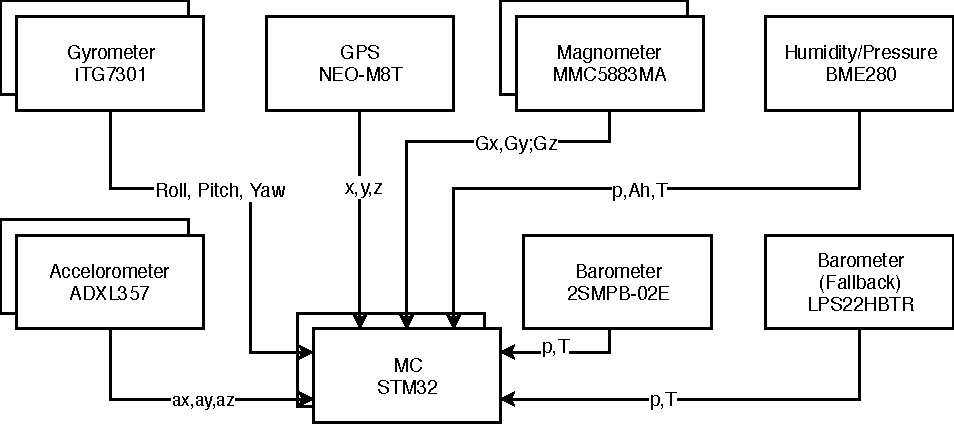
\includegraphics[width = \textwidth]{../BDADoku/Pictures/SensorNetworkAlt.pdf}
  \caption{Sensor Network}
  \label{fig:SensorNetwork}
 \end{figure}

 As mentioned above different sensors are used in this years competition and due to the assumption
 that in concept the same sensors will be used in the competitions coming they will act as the basis for the sensor fusion-
 This used sensors and their settings will be described in this chapter.

 % Insert more information about those sensors if I get to them...
 \subsection{Accelerometer}
 First of all, comes the accelerometer. This is a well established and widely used sensor. It measures the force which is applied on the sensor in the three
 space dimensions. 
 This years accelerometer is adxl357 which will be sampled at 1000 Hz. 
 
 \subsection{Gyrometer}
 The Gyrometer is needed to measure the posture of the Rocket. This is especially needed to determine if the rocket has a pitch angle. If so the pure
 acceleration on the z-axis can be calculated. The used gyrometer is ITG-3701 and it will also be sampled at 1000 Hz.
 
 \subsection{Barometers}
 Barometers are widely used in aviation, cause with a common pressure model the height can be calculated out of the measurements that the barometer takes.
 In this years competition three barometers are used. This are by name 2SMPB-02E and LPS22HBTR. They will be used with a sampling rate 100Hz and 50Hz. %Has to be checked
 In addition the Humidity/Pressure sensor BME280 does also measure the pressure which can be used in addition.
 
 \subsection{Temperature}
 The temperature is maybe needed to make the height out of the barometer better because most of the atmospheric model depend on the pressure as well as the temperature.
 This temperature will be provided by the different barometers which each posses a separate temperature sensor. 
 
 \subsection{Magnometer}
 Also there are two Magnometer in the sensor network \ref{fig:SensorNetwork}. These measure the strengths of the surrounding magentic field.
 This can be used to determine the direction regarding the north pole.
 Due to the fact that the algorithm that will be developed in this thesis does not include the X- and Y-Axis,
 these sensor will not be used for the sensor fusion.
 
 \subsection{GPS}
 For next years competition differential GPS will be implemented with the help of two $\mu$blocks modules.
 This taken measurements are more precise as the rest of sensors but are taken much slower on a rate like 1 Hz. Therefore the algorithm should takes
 those provided measurements and interpolate between them with the data from the other sensors.
 
 
 \section{Problems}
 Out of the research and the previous competition, different problems appeared that need to be addressed in this thesis to ensure an as good solution as possible.
 
 \subsection{Different Sensors}
 First of all there are different sensors which all do measure different values and have different parameters (precision, sampling time).
 So the algorithm has to use out the strengths of the different sensors to cancel out their individual weaknesses.
 Additionally, because this algorithm is system critical, it has to be reliable enough that it still is working properly if sensors failing. 
 
 \subsection{System Load}
 The cycling time will be around 1 ms on a embedded system. This time was chosen on the behalf that it would be difficult to get the exact needed cycling time on ensure the needed controllability of the rockets apogee.
 Therefore the system load that the algorithm can cause, has to be strongly limited, so that it can be run on this given system. 
 The system this year is an 32 bit Arm Processor which runs on 168 MHz, assumed that the algorithm has at maximum the half of a software cycle, the maximum given clock cycles are around 84 000.
 With this cycles the processor can do around 10000 simple calculation (addition, subtraction, multiplication, division),
 cause with its floating point unit it needs on average around 8.5 cycles per operation (load, calculate, store). 
 This number is just a rough assumption, which means that the final system load should not exceed this value by a great manner.
 
 \subsection{Precision}
 The Precision is after the system load the most critical attribute, if the algorithm does not get into the required accuracy the whole thing is more or less for nothing.
 The Control stated that the maximal error between the estimated and ground truth height should not exceed two meter. 
 This especially after the burnout at which the control with the air breaks will start.
 This accuracy is needed to proper control the aim of the apogee.
 
 \subsection{Settling Time}
 The settling time defines the time span when the first reliable measurements arrive after burnout until the estimation is into the required precision.
 This time span has to be small enough to ensure that the controlling has enough time to aim for the desired apogee. In the current system the burnout occurs 
 occurs around 3-3.5 seconds after ignition, whereas the whole flight upwards only takes around 23 seconds. Therefore the settling time needs to be around just
 one second so that the control has as much time as possible for the controlling.
 
 \subsection{Reliability}
 Due to given surroundings that come if a sensor package is placed into a rocket, the assumption has to be made that it will be possible that sensors fail in execution.
 Therefore the algorithm should provide the reliability of still working in a proper manner with some sensors failed. So that the execution of the controlling software
 in terms of functionality, but locally it has not to be as accurate as it would be with all sensors working.

 \subsection{Modularity}
 Although it can be assumed that the sensors will stay more or less they same over the next competitions, it is not ensured that exactly this sensors will be used.
 Therefore the presented algorithm should provide the possibility to exchange the sensors, as long as they resemble the old sensor in a feasible way.
 This will ensure a long term use of the provided algorithm.
 
 \section{Requirements}
 
 \begin{table}[h]
 \centering
 \begin{tabular}{|l|l|l|l|}	
 \hline	
 \bf{Requirement}   & \bf{Rating} & \bf{Aim} & \bf{Importance} \\ \hline
 System Load   & \# Calculation steps per loop & < 5000 & Critical \\ \hline
 Precision     & Error between estimation and ground truth  & < 2m in Z & High  \\ \hline
 Settling time & Time from first reliable to optimal estimation  & < 1 s &  High \\ \hline
 Reliability   & Functioning Estimation with \#failed sensors & 2-3 sensors & Medium \\ \hline	
 Modularity    & Effort needed to change a sensors & < 10 h work &  Desirable \\ \hline
 \end{tabular}	
 \caption{Requirements table}
 \label{tab:Requirements}
 \end{table}
 
 As seen in the table \ref{tab:Requirements} five requirements were drown out of the problem analysis. 
 First of all, there is critical requirement the system load. This is given as critical cause it is needed that the algorithm is small enough to be run on a embedded system.
 Any solution that would not fit this requirement would be pointless in the frame of this thesis.
 Secondly there are two requirements which are tied together, the precision and settling time.
 Where the precision describes what a optimal estimation is under the context of this thesis, the settling time relies on this to be defined.
 The desired precision will be needed to ensure a possible good control.
 
 \section{Desired Solution}
 The desired solution should met the given requirements as optimal as possible. While doing this it should also not be more complicated than needed
 to make a future use as easy as possible. Cause of this the modularity is an important requirement to ensure this.


\chapter{Approach}
\label{ch:Approach}

  This chapter discuses how the stated problem will be approached.
  This by stating the concepts which were developed for simulation.
  First the test concept and the concept to get the sensor models.
  After that the different system models as well as the different state estimated are discussed.
  
  \section{Verification}
  First of all the test concept has to be defined on which the developed algorithms will be tested.
  This is also be specially useful for the future competitions to test the adjusted algorithms which will be used there.
  For this the following concept which can be seen in figure \ref{fig:Verification} was developed.
  
  \begin{figure}[h!]
   \centering
   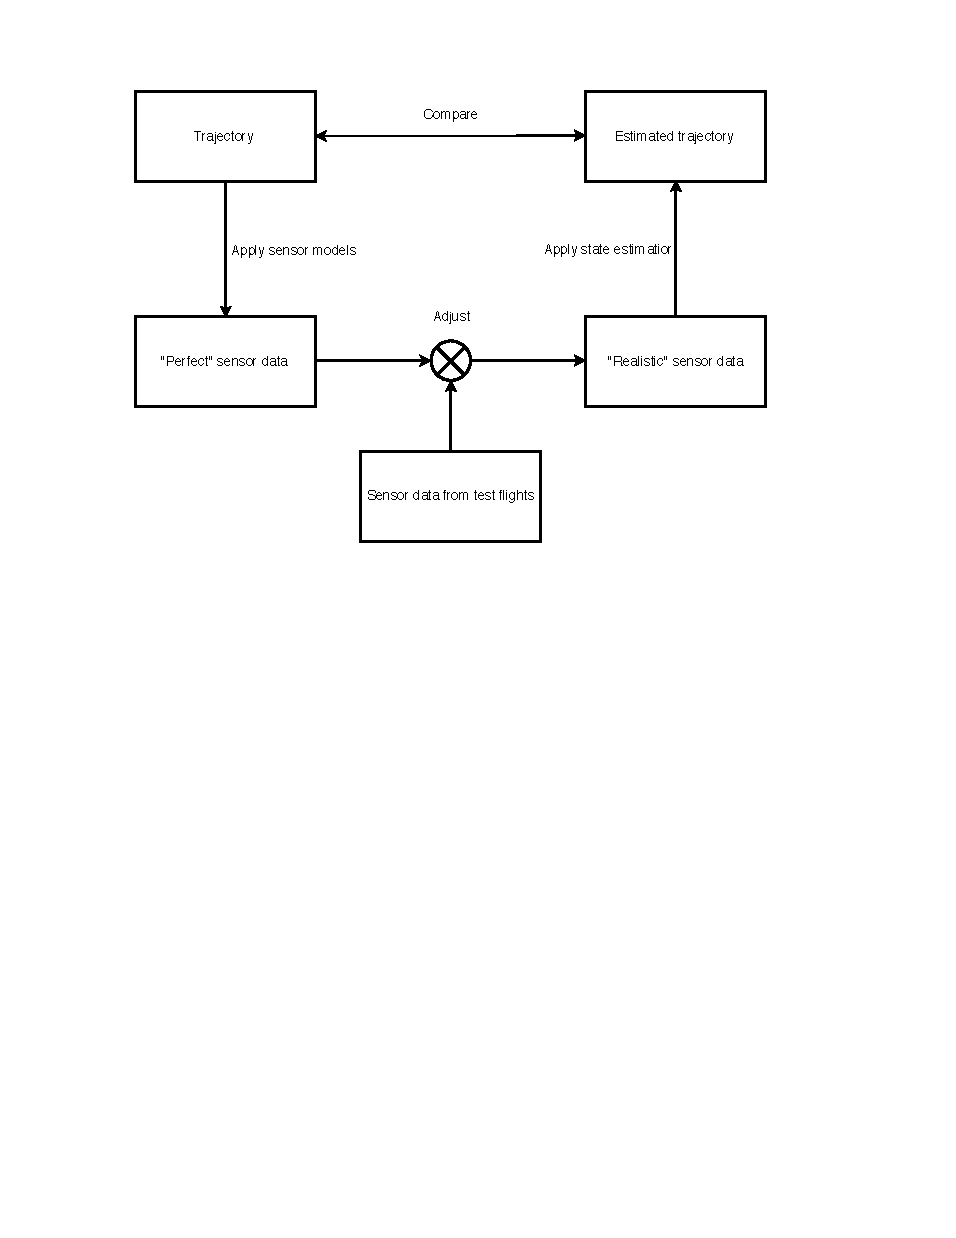
\includegraphics[width = \textwidth]{../BDADoku/Pictures/Verification.pdf}
   \caption{Verification Concept}
   \label{fig:Verification}
  \end{figure}

  The theory behind this is that a trajectory is generated by the simulation, which should resemble a real trajectory as good as possible.
  This function was provided by the simulation team of ARIS from the last years competition.
  Then this trajectory is applied on the sensor models which are discussed below.
  This generates so called perfect sensor data which would resemble the data provided by the sensor if they do not have any noise at all and the surrounding do preform as described. 
  After this the noise is applied which will also be developed later in this chapter, this will result in real sensor data. 
  This noise is drawn out of the sensor log data from the previous test flights.
  After the realistic sensor data is generated, it serves as the input to the different estimation algorithms.
  
  Then to verify the functionality of those algorithms, the estimated trajectory is compared against the generated trajectory.
  
  
  \section{Sensor models}
  As stated above the trajectory will be generated by the simulation. 
  This are just the information of the height, so the different sensor models have to be adjusted to get to the different needed data.
  The models are defined as follow.
  
  \subsection{Accelerometer}
  Perfect measuring from the accelerometer is in simple terms the two times deviation of the height.
  $$a = \frac{d^2h}{dt^2}$$
  This equals in the straight up acceleration. To get the acceleration which would be provided by an accelerometer,
  the pitch angle has to be calculated into this generated data.
  
  \subsection{Gyrometer}
  For the gyrometer there does not really exist a model with which those measurements could be generated.
  Therefore it has to be generated free hand by taking the gyrometer measurements from the testflights into account.
  It has also to be stated that only the pitch angle of the rocket which can be seen in figure \ref{fig:RocketPitchAngle} is for interest for this first sensor fusion implementation,
  So only this angle will be generated with random values which do drive towards a realistic value that was read out of the data from test flights.
  
  \begin{figure}[h!]
    \centering
    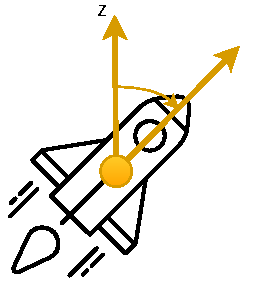
\includegraphics[width = 0.3\textwidth]{./Pictures/RocketSyMod.pdf}
    % RocketSyMod.pdf: 0x0 pixel, 300dpi, 0.00x0.00 cm, bb=
    \caption{Pitch angle visualisation}
    \label{fig:RocketPitchAngle}
  \end{figure}

  
  \subsection{Barometer}
  The barometer which are used in the aerospace usually provide the pressure in hecto Pascal as well as the temperature in degree Celsius.
  \subsubsection{Pressure}
  To generated the pressure data, the barometric height formula is used \cite{NASAEarthAtmosphereModel2015}.
  $$P = P0 \cdot (1- \frac{Tgrad\cdot h}{T0})^{\frac{M\cdot g}{R\cdot Tgrad}}$$
  \begin{tabbing}
  with: \= PO = Pressure at ground level \\
  \> TO = Temperature at ground level \\
  \> Tgrad = Temperature gradient for the actual weather condition \\
  \> M = Molar mass of Earth's air: 0.0289644 kg/mol\\
  \> g = Gravitational acceleration: 9.80665 m/$s^2$\\
  \> R = Universal gas constant: 8.3144598 J/mol/K\\
  \end{tabbing}

  This is more or less accurate till 11 000 meter under the condition that the Temperature gradient is determined correct. 

  \subsubsection{Temperature}
  The temperature depending on the height is a difficult subject because the temperature gradient is depending on the actual weather and the capacities of the air.
  So this gradient has to be determined before the start for each flight.

  $$T = T0 - Tgrad*h$$
  
  \subsection{GPS}
  The perfect GPS data is seen as the accurate height but with a slow sample rate around 0.5 to 2 Hz.
  This can simply be achieved by down sampling the height vector with the right factor.
  
  \section{Noise generation}
  To generate the different noises, first the noise from the test flight has to be extracted.
  If done so, a system can be calculated which represents a white noise filter that generates noises
  that has the same spectral power density as original noise. This process is visualised in figure \ref{fig:WhiteNoiseFilter}.
  
  \begin{figure}[h!]
 \centering
 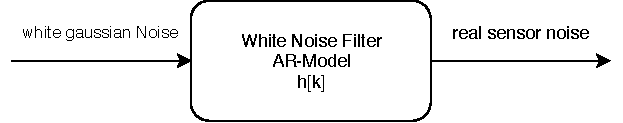
\includegraphics[width=0.5\textwidth]{./Pictures/WhiteNoiseFilter.pdf}
 % WhiteNoiseFilter.pdf: 0x0 pixel, 300dpi, 0.00x0.00 cm, bb=
 \caption{White noise filter concept}
 \label{fig:WhiteNoiseFilter}
\end{figure}
  
  
  For this the yule walker equation should come in handy to calculate a so called AR (auto regressive) model of the noise system.
  An AR model is a FIR (all pole) system which generates a random sequence with defined auto correlation $\gamma_{yy}$ out of white gaussain noise.
  
  $$ y[n] = \omega[n] - \sum_{k=1}^{N} a_k \cdot y[n-k]  $$
  
  The yule walker equations
  \begin{align*}
    \begin{bmatrix}
     \gamma_{yy}[0] & \gamma_{yy}[-1] & \dots & \gamma_{yy}[-N] \\
     \gamma_{yy}[1] & \gamma_{yy}[0] & \dots & \gamma_{yy}[-N+1] \\
     \vdots 		& \vdots 	& 	& \vdots	\\
     \gamma_{yy}[N] & \gamma_{yy}[N-1] & \dots & \gamma_{yy}[0]
    \end{bmatrix}
    & \cdot
    \begin{bmatrix}
     1 \\
     a_1 \\
     \vdots \\
     a_N   
    \end{bmatrix}
    = 
    \begin{bmatrix}
     \sigma^2_\omega \\
     0 \\
     \vdots \\
     0
    \end{bmatrix}
    \hfill
  \end{align*}
  \hfill
  estimate the coefficient $a_1 \dots a_N $ of the FIR system and the variance of the noise $\sigma^2_\omega $ which can be used to generate a random sequence which has the same auto correlation $\gamma_{yy}$ and therefore the same spectral capacities as the input sequence y.
  Because the AR model consists of an all pole filter, the noise should has to have a steady mean value preferably it should be zero mean.
  This way the estimated AR model from the yule walker equation can represent the real system at best.
  For this the mean value of the measurements should be calculated beforehand and then be subtracted to get there zero mean noises.
  The part of the mean values that represent noise and can then be added after the noise in generated to represent the real sensors as good as possible.
  
  \section{System Model}
  The system model to represent the rocket will be hold simple to reduce the system load as well as prevent non linearities.
  Also the important values to estimate are at first hand the vertical height and speed, so
  for a first implementation just variables that can bed used do determine those both will be used.
  This are mainly the height from the GPS, the vertical acceleration from the accelerometer
  as well as the pressure and temperature from the pressure sensors. In addition the pitch angle from the gyrometer is used to calculate the pure vertical acceleration.
  But even with such simplification there are different possible system description which have to be taken into account 
  to find the best suitable.
  
  \subsection{General State Space System}
  For this a quick view at general donation of a state space system. First there is the update function.
  $$ \dot{x} = A \cdot x + B \cdot u + G \cdot q$$
  Here the A matrix resembles how the system transmits over time by itself where the B matrix describes how input u does influence the system.
  In addition noise on the system can be described with the G matrix and the noise input q.
  The second equation is the output equation.
  $$ y = C^T \cdot x + D \cdot u + R $$
  Here the $C^T$ matrix describes how the state value from x effect the output while the D matrix describes how input directly effects output.
  The D matrix is zero in the most state space systems, because in reality there are not a lot of systems where the output directly and immediately reacts to input.
  Also the noise on the output (measurements) can be described with the R matrix.
  
  \subsection{Point Mass}
  The most simple possible model would be, that the rocket would be resembled as a simple point mass which flies perfectly vertical upwards.
  For this only three state variables would be necessary, the vertical acceleration, the vertical speed and the height.
  $$x = \begin{bmatrix}
  h_z\\
  v_z\\
  a_z
  \end{bmatrix} $$ 
  This would reduce the A matrix of the system to a 3x3 matrix with with only two 1 in it.
   Also the input matrix would be a zero matrix in this system because the input process 
  (power from the motor and drag force from the surrounding air) would be difficult to describe in a linear system.
  \begin{align*}
  A = \begin{bmatrix}
  1 & 0 & 0\\
  0 & 1 & 0\\
  0 & 0 & 0
  \end{bmatrix}
  & \hspace{1cm}
  B = \begin{bmatrix}
          0 \\
          0 \\
          0 \\
  \end{bmatrix}
  \end{align*}
  In addition the measurements which are taken from the sensor will be described as the system output (y vector). 
  So if the pressure from for example two barometers is calculated into the height beforehand it would result in the flowing output matrices.
 \begin{align*}
 y = \begin{bmatrix}
	  h_{GPS}	\\
          h_{p1}	\\
          h_{p2}	\\
          a_z
     \end{bmatrix}
    & \hspace{1cm}
 C^T = \begin{bmatrix}
         1 & 0 & 0	\\
	 1 & 0 & 0	\\
         1 & 0 & 0	\\
         0 & 0 & 1
        \end{bmatrix}     
  \end{align*}
  
  As normal in engineering such a simplification comes with a cost. With this system description the output from the barometer would have
  to be transformed into the height before they could be taken into the system. 
  Due to this the properties of these sensor could not be estimated correct because the value was transformed in a non linear way before it entered the system.
  In addition the same problem occurs with the accelerometer. If the rocket develops a pitch angle not equal to 0 during the asccending, it would be measured wrong.
  To counter this error, the measurements of the accelerometer would have to be weighted with the angle of the gyrometer before entering the system.
  This weighting is also non linear and the values of the gyrometer are not filtered, which would make the estimation even more uncertain.
  
  \subsection{Point Mass with Pressure}
  To taken into account to problem stated above, pressure can be taken into the state vector and therefore be estimated.
  $$ x = \begin{bmatrix}
  h_z\\
  v_z\\
  a_z\\
  p\\
  \end{bmatrix} $$ 
  While this solves the problem stated above, it also produces a new. The system model can only describe linear dependencies between the state variables,
  but the relation between the pressure and the height is clearly non linear in each atmospheric model.
  This dependency can be linearized, but if done so, it does resemble the atmospheric model with less accuracy.
  This linearisation can be used to interpolate between the barometer measurements so the actual pressure is available at any loop iteration.
  This results in a 4x4 A matrix and also a zero B vector for the dynamics equation which look like this:
  \begin{align*}
  A = \begin{bmatrix}
         1    & 0 & 0 & 0    \\
         0    & 1 & 0 & 0    \\
         0    & 0 & 0 & 0    \\
         0    & KP_v & 0 & 0\\
        \end{bmatrix}
        & \hspace{1cm}
    B = \begin{bmatrix}
       0 \\
       0 \\
       0 \\
       0
      \end{bmatrix}
  \end{align*}  
  
  This would also inflect on the output matrices which do then contain the pressure directly.
  In addition the height calculated from the pressure can be inserted as additional measurements to include them into the estimation.
  
  \begin{align*}
   y = \begin{bmatrix}
        h_{GPS}	\\
        h_{p}	\\
        a	\\
        p_1	\\
        p_2	
       \end{bmatrix}
       & \hspace{1cm}
  C^T = \begin{bmatrix}
       1 & 0 & 0 & 0 \\
       1 & 0 & 0 & 0 \\
       0 & 0 & 1 & 0 \\
       0 & 0 & 0 & 1 \\
       0 & 0 & 0 & 1 
      \end{bmatrix}
  \end{align*}
  The input matrix stays except of an additional dimension the same as above.

  \subsection{Point Mass with Angle and Pressure}
  The same solution as above can also be applied for the pitch angle. 
  But its linearization and dependencies  more complicated and can therefore not be directly put into the system equation.
  This would change the state vector from above into the following.
  $$ x = \begin{bmatrix}
  h_z\\
  v_z\\
  a_z\\
  p\\
  \varphi_{pitch}\\
  \end{bmatrix} $$
  This would extend the dynamic part for A into a 5x5 matrix while the B matrix still would be a zero vector.
  \begin{align*}
  A= \begin{bmatrix}
        0 & 1 & 0 & 0 & 0 \\
        0 & 0 & 1 & 0 & 0 \\
        0 & 0 & 0 & 0 & 0 \\
        0 & Kp_h & 0 & 0 & 0 \\
        0 & 0 & 0 & 0 & 0 \\
        \end{bmatrix}
  & \hspace{1cm}
  B = \begin{bmatrix}
             0 \\
             0 \\
             0 \\
             0 \\
             0 \\
        \end{bmatrix}
  \end{align*}
  
  In addition the output matrix and the y vector will also change to adjust for the gyrometer measurements.
  \begin{align*}
   y = \begin{bmatrix}
        h_GPS \\
        h_p \\
        a \\
        p_1\\
        p_2\\
        \varphi_{pitch}
       \end{bmatrix}
       & \hspace{1cm}
       C^T = \begin{bmatrix}
        1 & 0 & 0 & 0 & 0 \\
        1 & 0 & 0 & 0 & 0 \\
        0 & 0 & 1 & 0 & 0 \\
        0 & 0 & 0 & 1 & 0 \\
        0 & 0 & 0 & 1 & 0 \\
        0 & 0 & 0 & 0 & 1 \\
        \end{bmatrix}
  \end{align*}
  With this the pitch angle would be some sort of real time low pass filtered.
  This solution would take all measurements available for the needed values into account.
  It would also keep the calculation in the system as simple and linear as possible.
  
  \subsection{Discretisation}
  The system stated above are all in continuous time state space description. 
  For implementation on a discrete time system like a micro controller they have to be discretisized.
  Those discrete matrices which will be denoted with an additional lowercase d (A -> Ad).
  The general state space discrete description with noise looks as follow.
  $$ x[k+1] = Ad\cdot x[k] + Bd\cdot u[k] + Gd\cdot Q[k] $$
  $$ y = C \cdot x[k] + D\cdot u[k] + R[k] $$
  As it can see only the A, B and G matrices have to be discredited this because 
  the matrices used in the second equation are only there for scalar adjustment for the output
  and should therefore not contain any time depending calculation.
  The Ad matrix can be calculated with the the following formula.
  $$ Ad = e^{A\cdot Td}$$
  Where Ts stands for the sampling time of the system which would be 1 millisecond on the system developed for this thesis.
  In addition there are two known ways to calculate the other needed discrete matrices Bd and Gd.
  \begin{itemize}
   \item $$ Bd = Ad \cdot B $$
	 The first one resembles a perfect sampling which is equal to a multiplication with a dirac impulse (the value is measured in a infinite small instant).
	 This calculation is rather further from the reality because no sensor can measure with perfect dirac impluse.
	 The great advantage of this method on the other hand is its simple calculation.
   \item $$ Bd = \int_0^{Ts} e^{A\cdot v}\cdot B \ dv $$
	 This version does resemble a zero order hold likewise measurement which is done by most sensors so it is more realistic than the first version.
	 It comes at the cost that the calculation is more difficult \cite{DavidWSchultz2004}.
  \end{itemize}

  Both version have to be tested in the simulation to see if the additional effort for the second version pays of enough.
  
  \section{State estimator}
  There are many possibilities to do sensor fusion. first of all an all new algorithm could be developed which accesses the 
  stated problems directly. While this solution would be preferable regarding the efficency, the 
  time and knowledge needed for this task would exceed the resources given in this thesis by far.
  Also as stated in chapter \ref{ch:Introduction} a lot of theoretical as well as practical pre work is
  already done and therefore should be used. 
  So following different possible approaches with there pro and cons will be discussed. 
  
  \subsection{Kalmanfilter}
  First of all the traditional discrete Kalmanfilter has to be discussed as it provides the base for the most known state estimator.
  Its structure provides the optimal estimation of the standard deviation estimation error as long as the noises are Gaussian
  and the observed system can be described by linear differential equations.
  But there lies the problem, a physical system is most often not linear.
  Also the estimated system as well as its variances over the time have to be known to provide this optimal estimation.
  If the noise matrices of the system are static, the filters gain matrices aim for a fix value and can therefore be calculated in beforehand.
  This reduces the computational effort by a significant amount. \cite{DavidWSchultz2004}.
  It should be mentioned that even if the noise is not Gaussian, the Kalmanfilter is still the best
  linear estimator as long as the system and its properties are well known \cite{SimonDan2006Ose:}.
  To summarise it, the discrete Kalmanfilter is a simple to understand and adjust state estimator in comparison to the following.
  
  \subsection{ROSE}
  The ROSE(rapid ongoing stochastic estimator) is in simple terms three Kalmanfilters in one.
  Where the main filter is used as a normal Kalmanfilter like stated above, the additional two are used to estimated the 
  the system noise as well as the measuring noise. Therefore this sensor preforms better than the traditional Kalmanfilter
  if those noises change over time in a not known fashion and has therefore be estimated.
  Due to this, this sensor needs more computational effort to preform this estimations \cite{DavidWSchultz2004}. 
  
  \subsection{Extended Kalmanfilter}
  The extended Kalmanfilter provides additional parts to better access non linearity in the observed system.
  This by not estimating the state of the system but by estimating the linearized change of the state 
  to the next coming state. For this the systems equations have to be derived around the current nominal point in every estimation state.
  This is some sort of Bootstrap solution because the nominal point on which the derivation happens are estimated in the process and
  this estimates are then used to estimate the change between this estimation and the next.
  Therefore the computational effort exceeds even further because each function has to be deviated at each loop iteration \cite{SimonDan2006Ose:}.
  
  \subsection{Unscented Kalmanfilter}
  The unscented Kalmanfilter takes the unscented transformation in use to calculate the different interpolating steps.
  The unscented transformation uses a test set of points around the current state and calculates the new values for them using the functions which represent the system.
  Out of these new values calculated from the test set is now the new state estimated by weighting those new values depending on there probability of occuring. 
  With this the state function do not have to be linearized and therefore the the estimation is most time better than that of the extended kalmanfilter.
  But for this the unscented Kalmanfilter needs also to apply the unscented transformation onto the state vectors in each iteration
  and does therefore need even more computational effort \cite{SimonDan2006Ose:}.
  
  \subsection{H$\infty$ filter}
  The H$\infty$ filter is a more diverse approach then the ones described above.
  It was developed to access the problem when the to be observed system especially its noise is not well known.
  In other words it was developed to resemble an as robust as possible state estimator.
  In addition its stability can be easier guaranteed that with a Kalmanfilter.
  For this it consists of additional tuning parameters which makes it more complicated ti use.
  Also in contrast to the Kalmanfilters the H$\infty$ filter minimises the worst-case estimation error 
  in stand of the standard deviation of the estimation error \cite{SimonDan2006Ose:}.
  
  \newpage
  \section{Choosing}
  If the requirements table \ref{tab:Requirements} is taken into the consideration of finding
  the optimal solution, two main requirements occur that define this decision.
  First the system load is a critical requirements and has therefore to be addressed in this process.
  Also for the requirement of modularity the algorithm should be as simple as possible.
  If taken in regard that the system is more or less well known and that the noise can be
  determined with the simulation and the log data from previous test flights,
  a normal Kalmanfilter seems to be the most fitting solution.
  This because the performance of the rocket and the sensor should stay the same during
  each flight. 
  
  \subsection{Functioning}
  Since the best fitting state estimator was chose. Its detailed functioning shall be described here.
  This algorithm works in four main equations which can be divided into prediction and correction steps figure \ref{fig:Kalmanfilter}.

  \begin{figure}[h!]
    \centering
    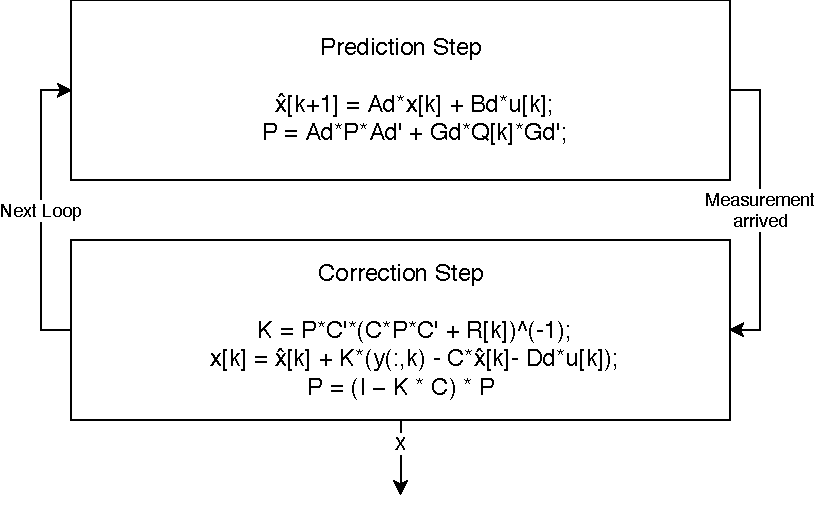
\includegraphics[width = \textwidth]{../BDADoku/Pictures/KalFIlFunc.pdf}
    \caption{Kalmanfilter}
    \label{fig:Kalmanfilter}
  \end{figure}

  \subsubsection{Prediction Step}
  The prediction equations take the currently values of the state vector ($x[k]$)
  and uses the time depending system model part (Ad) to predict the state values for the next time step $\hat{x}[k+1]$.
  The hat denotes that this value is an assumption.
  This with the equation: $$ \hat{x}[k+1] = Ad\cdot x[k] + Bd\cdot u[k] $$
  In addition the certainty matrix (P) is estimated with the same tactic, which means that it is calculated how trustworthy those predictions are.
  $$ P = Ad\cdot P\cdot Ad^T + Gd\cdot Q[k]\cdot Gd^T$$
  For this the system noise is used, so with the help of the Q matrix it can be stated how well known the system is in this
  time step.

  \subsubsection{Correction Step}
  If the measurements arrive those will be used can be used in the correction step to correct the prediction.
  First the Kalmangain (K) is calculated with the equation.
  $$ K = P\cdot C^T\cdot (C \cdot P \cdot C^T + R[k])^{(-1)} $$ 
  This uses the P matrix from the prediction step as well as the R matrix which represents the noise on the measurements (how certain the values from the measurements are).
  K is then used in the equation. $$x[k] = \hat{x}[k] + K\cdot (y[k] - C\cdot \hat{x}[k]-Dd\cdot u[k])$$
  With this the measurement is used to correct the predicted value of the state vector with there uncertainties taken into account \cite{DavidWSchultz2004}. 
  In the last equation $$P = (I − K * C) * P $$ the certainty matrix is corrected with the help of the kalman gain and the estimated certainty matrices.
  
  For this the matrices for the system models (Ad,Bd,C,D), the measurements noise (Q,Gd) as well as the system noises (R) have to be defined.
  
  
  
  

\chapter{Implementation}
\label{ch:Implementation}
%How it will be Implemented

%\section{Tipps/Notes}
%make plots from the different sensors and the log data to show how it was 
%produced an how it resembles the real data.
%The simulation itself is implemented in Matlab as different .m files.

\section{Sensor Models}
How the concept of the different sensor models work is described in chapter \ref{ch:Approach}.
Following here, the implementation which is used in the simulation will be stated in detail.
First in general for all sensors, following by the different characteristics of each sensor.

\subsection{Perfect Sensor}
In general, the perfect sensor data are calculated like stated in chapter \ref{ch:Approach}.
In figure \ref{fig:GeneratedPerfectSensor} those generated sensor data as well as the trajectory used for this can be seen.

\begin{figure}[h!]
 \centering
 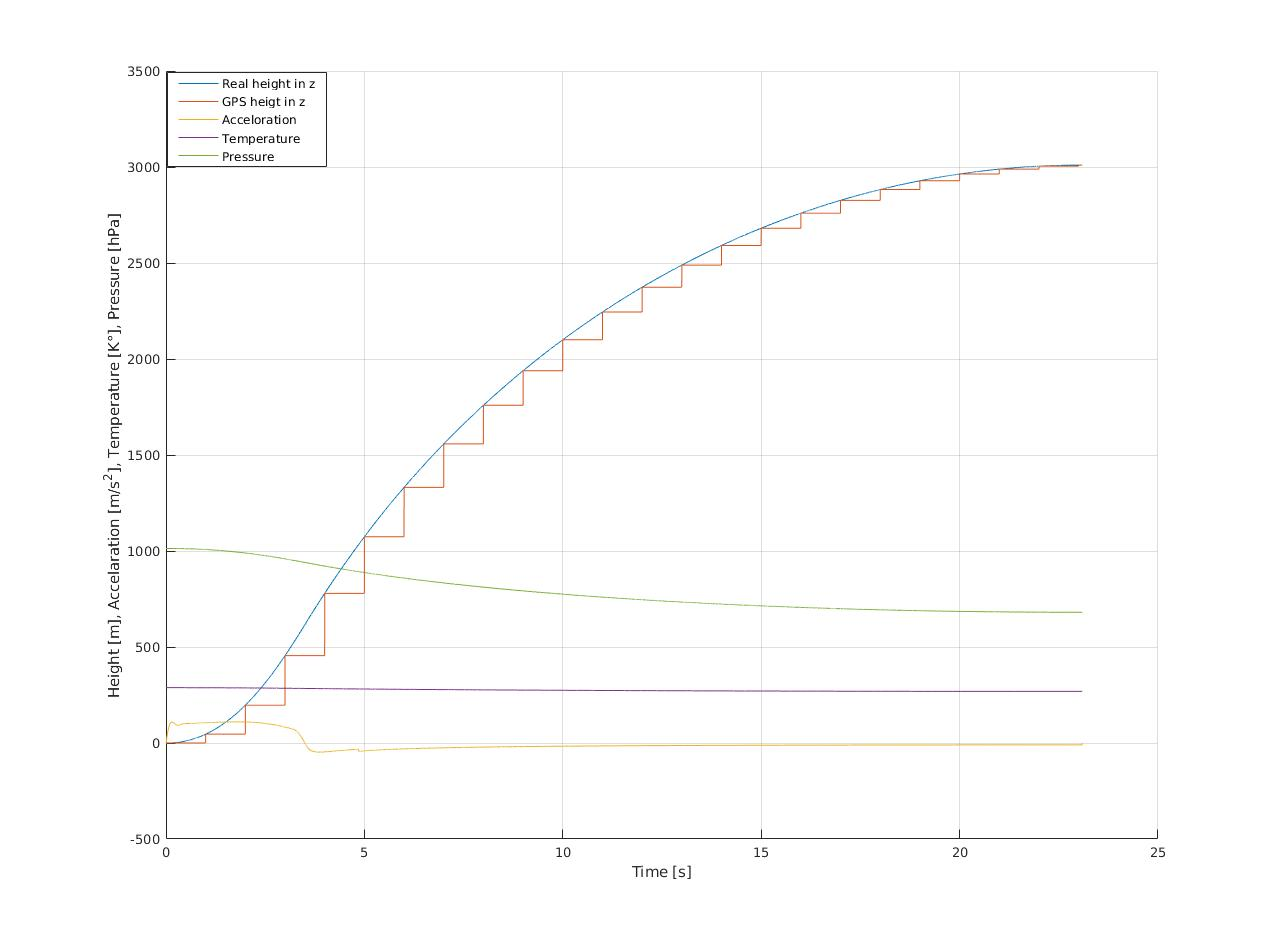
\includegraphics[width=0.8\textwidth]{./Pictures/GeneratedSensorData.jpg}
 % GeneratedSensorData.jpg: 0x0 pixel, 300dpi, 0.00x0.00 cm, bb=
 \caption{Generated sensor data}
 \label{fig:GeneratedPerfectSensor}
\end{figure}

\subsubsection{Accelorometer}
Due to the fact that whole simulation works with discreet time stamps, the derivative of the height can not be done formally.
So it is done by calculating the difference in each data point to the next and then weight those by the delta in time between them.
This has to be done two times to get from the height to the acceleration.
The unit for the acceloration in this simulation is meter per second squared.

\subsubsection{Gyrometer}
As stated before the pitch angle can not be directly generated.
But if the  data from the test flights are visited. It can be seen that the angle stays more or less the same wile the motor is burning.
This make sense because during this time the main acceleration comes from one determinet direction and stabilices the rocket.
After the burnout the pitch angle does change more or less randomly depending on strength and direction of the wind that hits the rocket.
To reanimate this the values are generated randomly and the low pass filtered with a moving average filter to represent that behaviour.
While doing this the random values are kept small during the burning of the motor and exceed afterwards to higher values.

\subsubsection{Barometer}
The measurements from the barometer are depending on the formula stated in chapter \ref{ch:Approach}.
For reasons of simlicity the start pressure is choosen as the mean pressure at sea level which is 1013.35 hPa.
Also the temperature at the beginning is chosen as 288.15 degree Kelvin (15 degree Celcius) which also represents the mean value on the sea level.
At least the temperature gradient is - 0.0065 °/m which is a common used value.
For the state estimation in a test flight those values have to be determined before the start.

\subsubsection{GPS}
As stated in chapter \ref{ch:Approach} the GPS signal is just the height with a different sampling time. 
To maintain the vectors length which simplifies the later use in the estimation algorithm,
the signal is acquired with a zero order hold conversion instead of a down sampling. 

% Add code for the zero order Holde convertion

\subsection{Noise}
To generate the noise out of the data from the test flight, this has first to be extracted.
It is assumed that the noise on the data is different depending on the state of the rocket (before Icognition, during motor burning, after burnout till parachute ejection),
but it should have more or less the same properties between those events.
Depending on this, the data vector have first to be separated in those different sections.
For this the accelorometer measurements are iterated to find the time stamps on which those events happen like in figure \ref{fig:AccelerationMarks}.

%% picture of acceloration of z axis with icognition, burnout and parachute ejection are marked
\begin{figure}[h!]
 \centering
 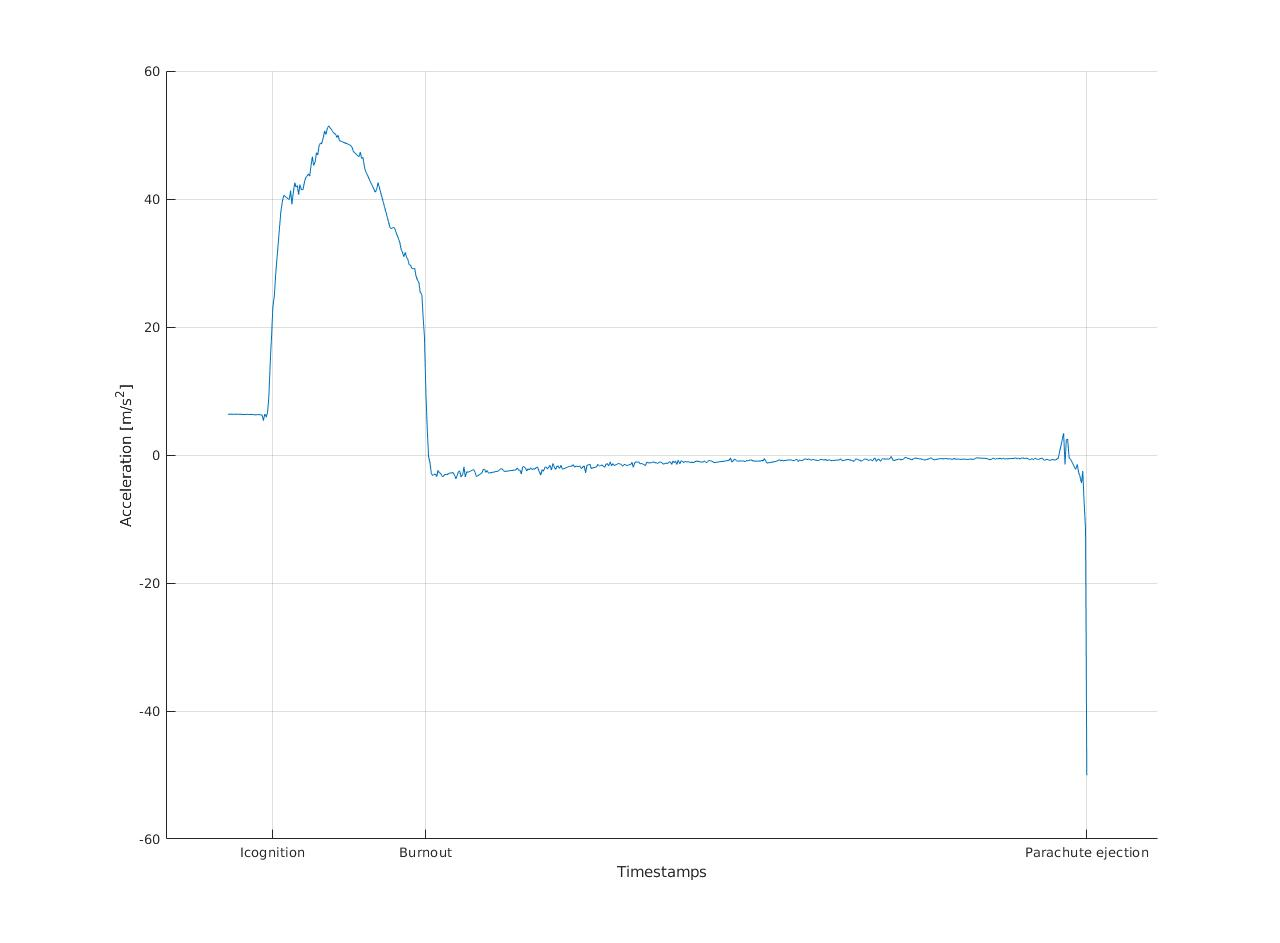
\includegraphics[width=0.8\textwidth]{./Pictures/AccelerationMarks.jpg}
 % AccelerationMarks.pdf: 0x0 pixel, 300dpi, 0.00x0.00 cm, bb=
 \caption{Timestamps drawn out of acceleration measurements}
 \label{fig:AccelerationMarks}
\end{figure}


If done so, polynoms are fitted on this measurements with the least squared error method.
Those polynoms represent the function which is assumed to be the noiseless data with possible offsets.
So if now the test flight data is subtracted by those polynomial curves which results in the noise without a mean.
From this point on this noise can be examined on its parameters, like the power density, the probability distribution and the variance figure \ref{fig:PF_AC_HIST_Accel}.

%% pictue of autocorrelation, histogramm etc from sensor data noise
\begin{figure}[h!]
 \centering
 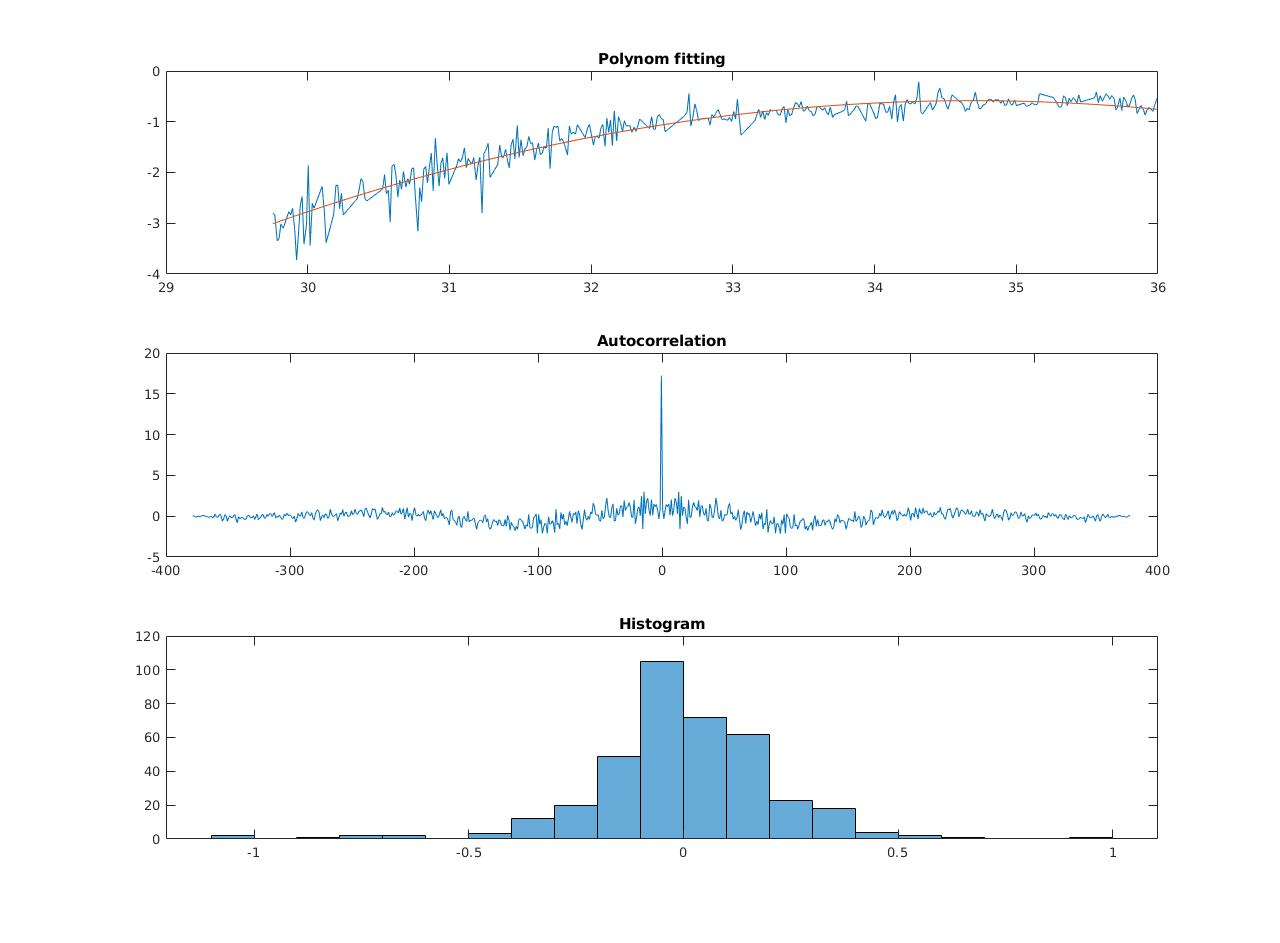
\includegraphics[width=0.8\textwidth]{./Pictures/PF_AC_HIST_Accel.jpg}
 % PF_AC_HIST_Accel.jpg: 0x0 pixel, 300dpi, 0.00x0.00 cm, bb=
 \caption{Polyfit Autoccorellation and Histogramm}
 \label{fig:PF_AC_HIST_Accel}
\end{figure}


This noise data can now used tho solve the yule walker equation to get an AR-model.
For this the aryule function in can be used which estimates an AR-model of the order N as well as the variance directly out of the noise vector.
But first, the data has to be resampled so that the AR-models can be used proper in the simulation.
With those AR-models, the noise can be regenerated by filtering white noise with the correct variance.
This generated noise can now be compared to the noise form the test flight data.

%% picture of pwelch plot from both noise vectors
\begin{figure}[h!]
 \centering
 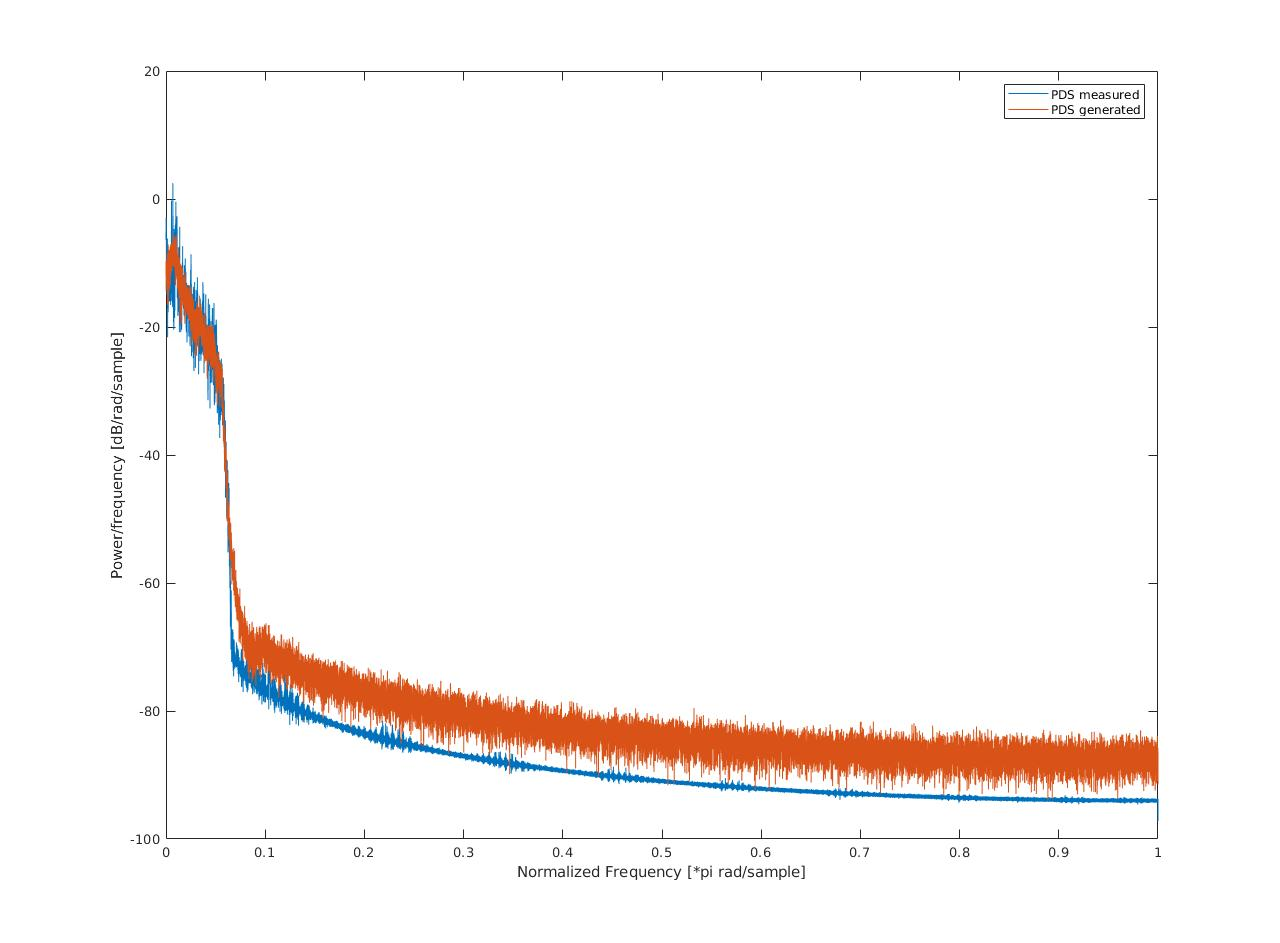
\includegraphics[width=0.8\textwidth]{./Pictures/PDSnoise.jpg}
 % PDSnoise.jpg: 0x0 pixel, 300dpi, 0.00x0.00 cm, bb=
 \caption{PDS form the measured and generated noise}
 \label{fig:PDSNoise}
\end{figure}


As seen in figure \ref{fig:PDSNoise} those noise resemble each other in their power density spectrum much more than the white noise would.
So this AR-model is exported to the simulation script and can be used there to generate the real sensor data.

\subsubsection{Accelorometer}
The noise which is on the accelorometer is special because it often has a drift which results in a more or less constant offset.
To recreate this, the offset can be estimated from the test flight data.
Especially the data before the ignition are help full, because the value that should be measured is known.

\subsubsection{Gyrometer}
For the gyrometer noise a separate script was written to calculate the proper pitch angle and filter out the offset before generating the AR-model.
This because the gyrometer measurements which are available are in degree per second and have therefore to be integrated before they resamble the correct pitch angle.
In addition it is complicated to define which part of the measurements are noise and which is the ground truth.
It was found that the estimated AR- model could not regenerated the noise with proper capacities.
Because of that, the noise has to be low pass filter afterwards to resemble the noises better.
For this task a IIR filter of order 200 was found best.
Therefore those measurements have to be properly handled.

\subsubsection{Barometer}
First there are two or more barometer which sample on different frequencies ant have therefore also different accuracy's.
This is represented in the way that the variance of the noise from the slower sampled barometer is kept on a smaller value,
than that of the sensor which is faster sampled.

\subsubsection{GPS}
The GPS noise capacities were found with measurements that were taken for a longer time period while the GPS receiver at the same place.
So the noise will have the same capacities over the whole flight.
This due to the assumption that the GPS measurements should be independent from the motors vibration and the rockets posture changes.
This should be suitable as long as the receiver does not lose its fix.

\newpage
\subsection{Real Sensor}
To now generated the real sensor data, the different noises have to be generated like stated above.
For this a vector of normal distributed random values is generated and multiplied by the square root of the corresponding variance.
This white noise is now filtered by the corresponding AR-model and can then be added onto the corresponding perfect sensor data.
This now results in the real sensor data.

\subsubsection{Accelorometer}
\begin{figure}[h!]
 \centering
 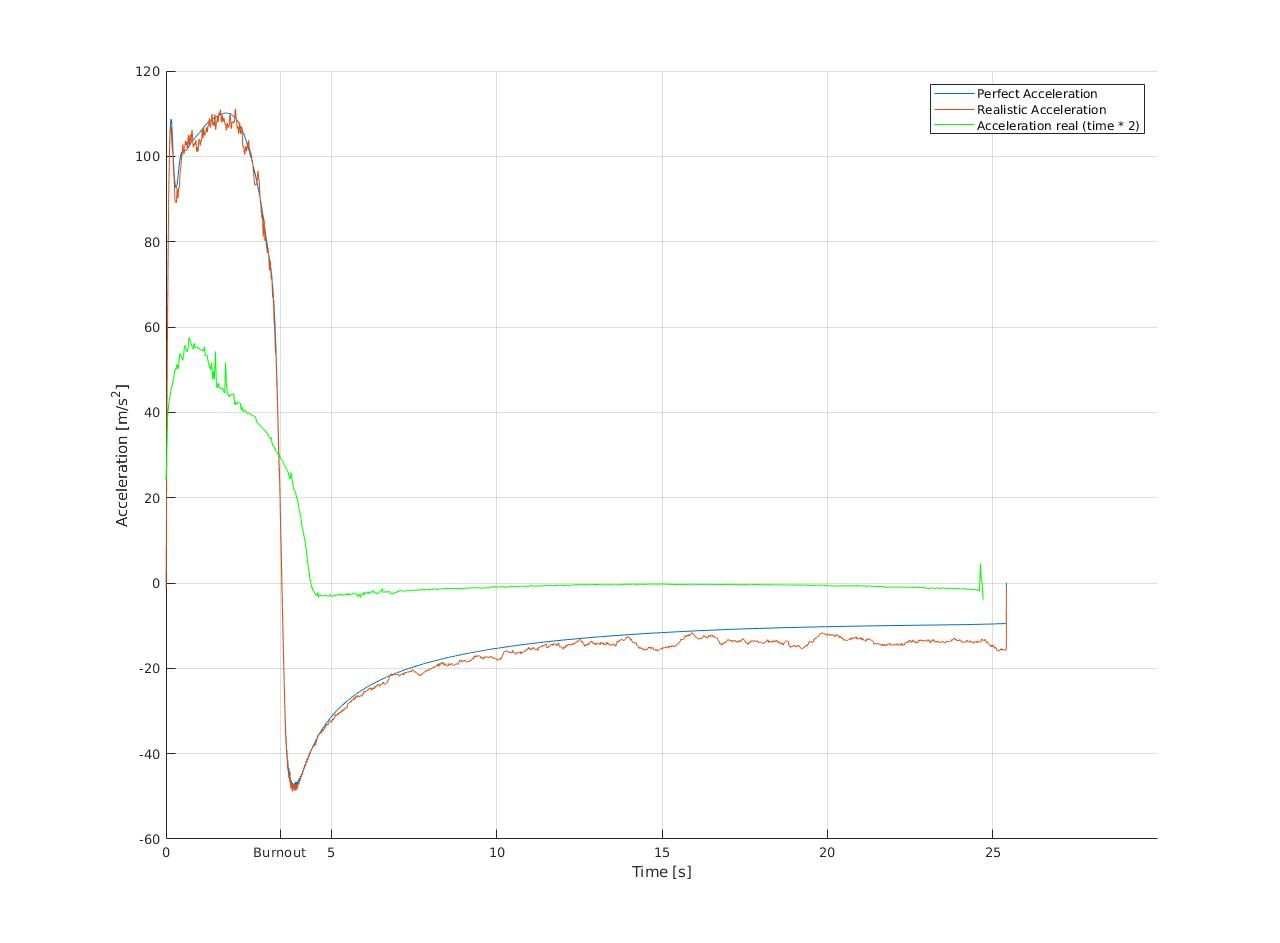
\includegraphics[width=0.8\textwidth]{./Pictures/AccelPerfVSReal.jpg}
 % AccelPerfVSReal.jpg: 0x0 pixel, 300dpi, 0.00x0.00 cm, bb=
 \caption{Plot of perfect acceleration vs realistic vs measured}
 \label{fig:AccelPerfVsReal}
\end{figure}
In figure \ref{fig:AccelPerfVsReal} the different generated values as well as the data from a test flight can be seen.
The time vector from the test flight was stretched by the factor two to make the observation easier.
Also it has to be said that the test flight was with a smaller rocket which flew only at an apogee of around 300 meters.
This explains why the acceleration is as great as in the generated data and why the time vector had to be stretched.
But the plot shows that the noise as well as the perfect data resemble the acceleration from the test flight in a appropriate way.

\newpage
\subsubsection{Gyrometer}
\begin{figure}[h!]
 \centering
 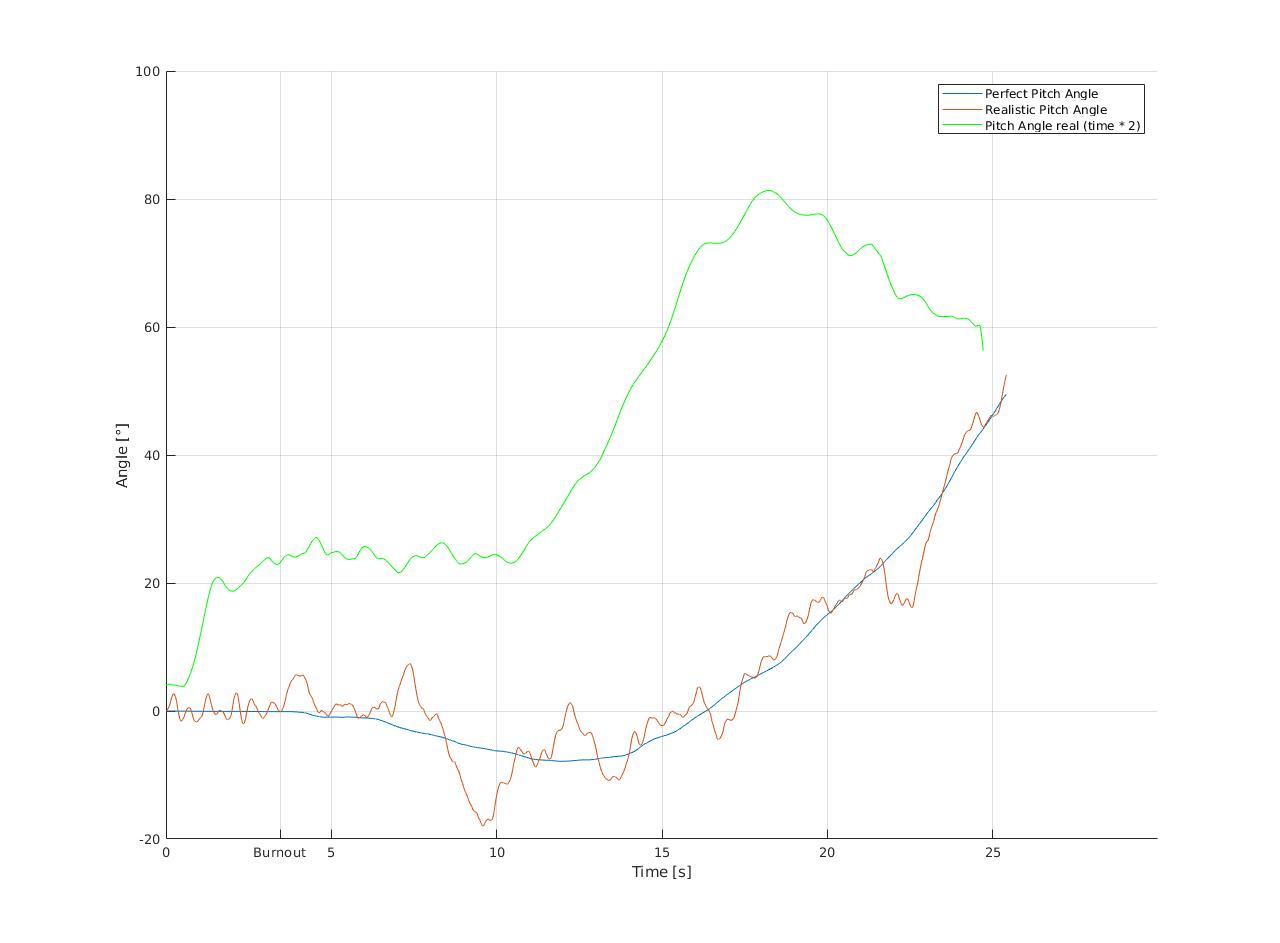
\includegraphics[width=0.8\textwidth]{./Pictures/PitchPerfVSReal.jpg}
 % PitchPerfVSReal.jpg: 0x0 pixel, 300dpi, 0.00x0.00 cm, bb=
 \caption{Plot of perfect gyrometer vs realistic vs measured}
 \label{fig:PtichPerVSReal}
\end{figure}
Figure \ref{fig:PtichPerVSReal} shows the generate gyrometer data.
Like in the acceleration plot the time vector from the test flight data was adjusted for better observability.
It should also be explained due to the proberty of the pitch angle (more or less random depening ond air current etc) that the generated realistic pitch angle must not resamble the measured angle in its specific value.
Important is in first hand that the noises have the same capacities which they do.
Also it can be seen that the assumption that the angle does no change great during the burning of the motor is despite a quick change at the start appropriate.

\newpage
\subsubsection{Barometer}
\begin{figure}[h!]
 \centering
 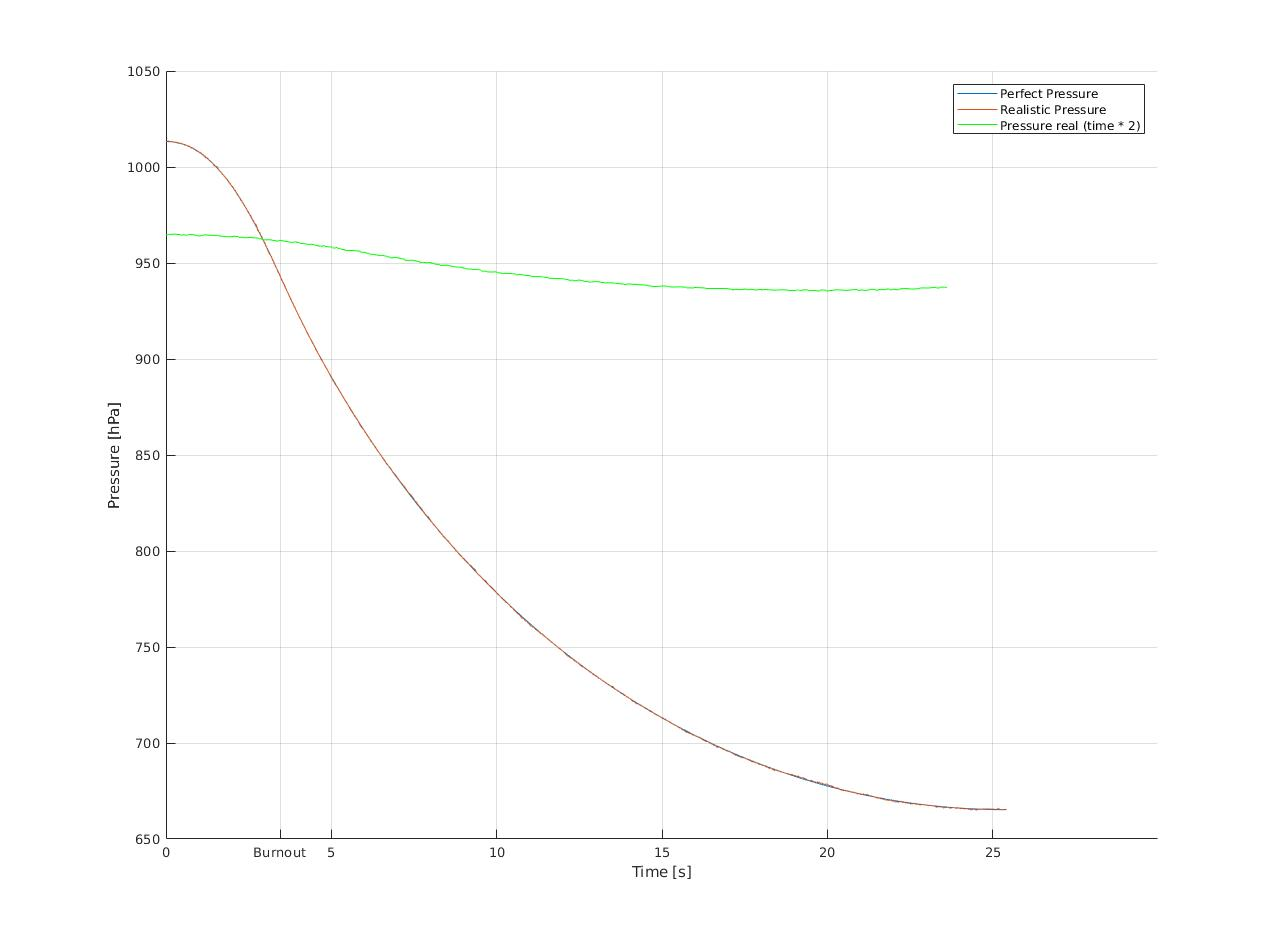
\includegraphics[width=0.8\textwidth]{./Pictures/PressurePerfVSReal.jpg}
 % PressurePerfVSReal.jpg: 0x0 pixel, 300dpi, 0.00x0.00 cm, bb=
 \caption{Plot of perfect barometer vs realistic vs measured}
 \label{fig:PressurePerfVSReal}
\end{figure}
The realistic pressure measurements from a barometer are shown in the figure \ref{fig:PressurePerfVSReal}.
The noise itself does not to see as it would have a great impact on the perfect data.
But this decieves because the pressure does change by around 350 hecto Pascal during the upflight
and therefore the changes from the noise which are around 1 to 3 hecto Pascal can not be seen that good.
The comparison with the real measured data (in the figure also with a stretched time vector) shows that generated realistic measurement data does resemble real measurements.

\newpage
\subsubsection{GPS}
\begin{figure}[h!]
 \centering
 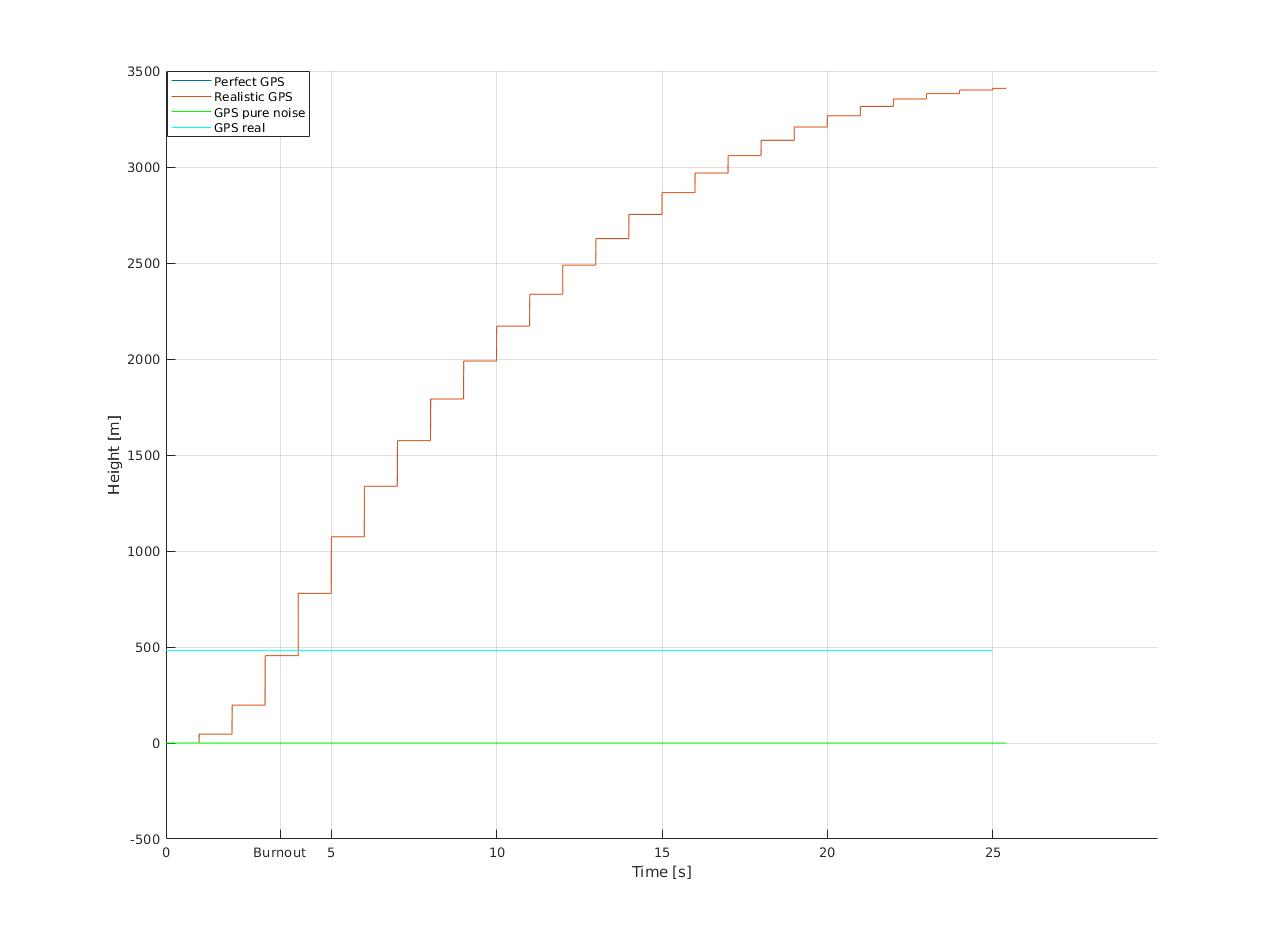
\includegraphics[width=0.8\textwidth]{./Pictures/GPSPerfVSReal.jpg}
 % GPSPerfVSReal.jpg: 0x0 pixel, 300dpi, 0.00x0.00 cm, bb=
 \caption{Plot of perfect GPS vs realistic vs measured}
 \label{fig:GPSPerfVSReal}
\end{figure}
At least the generated GPS measurements can be observed in the figure \ref{fig:GPSPerfVSReal}.
In this plot the pure generated noise was also plotted because as it can be seen it has real slow properties.
For the comparison the measurements which were taken from a fixed position are plotted (because there were no usable GPS data from a test flight avaiable during the term of this thesis).
It can be seen that the test data does also resemble the noise from the generated data.


\section{State Estimation}
As stated the used state estimator is a kalman filter with dynamic noises in the measurements as well in the systems.
For this the noise matrices as well as the used loop is described below.

\subsection{System Model}
The models are modelled as stated in chapter \ref{ch:Approach} but from this different uses can be made out of this.
For this simulation 8 models were implemented with each different capability.

Due to this, these different implementation are tested and evaluated in the next chapter.
\subsection{Adjustment}
Taken into account the above stated noise capacities of the measurements there were new systems developed which should hopefully result in better results.
\subsubsection{Offset}
The main adjustment is the inclusion of acceleration offset into the state vector.
This is a common tactic used so that the state estimator can estimate the actual offset and therefore the impact of the offset can be minimised \cite{DavidWSchultz2004}.
Therefore the state vector of a point mass would look like this.
$$ x = \begin{bmatrix}
        h_z \\
        v_u \\
        a_z \\
        a_{offset} \\
       \end{bmatrix}
$$
While the dynamic matrices A and B would stay the same apart form an additional dimension of zeros for the acceleration offset state variable.
\begin{align*}
 A = \begin{bmatrix}
      0 & 1 & 0 & 0 \\
      0 & 0 & 1 & 0 \\
      0 & 0 & 0 & 0 \\
      0 & 0 & 0 & 0
     \end{bmatrix}
     & \hspace{1cm}
 B = \begin{bmatrix}
      0 \\
      0 \\
      0 \\
      0
     \end{bmatrix}
\end{align*}
The y vector would stay the same while the output matrix $C^T$ will be adjusted so that both acceleration in the state vector are added into the accelerometer measurements.
\begin{align*}
 y = \begin{bmatrix}
      h_{GPS} \\
      h_{p1} \\
      h_{p2} \\
      a
     \end{bmatrix}
     & \hspace{1cm}
 C^T = \begin{bmatrix}
      1 & 0 & 0 & 0 \\
      1 & 0 & 0 & 0 \\
      1 & 0 & 0 & 0 \\
      0 & 0 & 1 & 1
     \end{bmatrix}
\end{align*}

\subsubsection{Acceleration as Input}
An additional adjustment would be to consider the measured acceleration of the rocket as input into the system.
This should result into a system which could react faster to changes in the acceleration.
For this the measurement noise of the accelerometer would have to be placed in the system noise matrix 
and therefore no additional system noise can be modulated.
For a point mass this would result in the following system matrices.
While the state vector and the A matrix would stay the same, the B vector would have to be adjusted like this.
$$ B = \begin{bmatrix}
        0 \\
        0 \\
        1
       \end{bmatrix}
$$
In addition the y vector would lose its acceleration measurements and the output matrix $C^T$ the corresponding dependencies.
\begin{align*}
 y = \begin{bmatrix}
      h_{GPS} \\
      h_{p1} \\
      h_{p2} \\
     \end{bmatrix}
      & \hspace{1cm}
 C^T = \begin{bmatrix}
        1 & 0 & 0 \\
        1 & 0 & 0 \\
        1 & 0 & 0 \\
       \end{bmatrix}
\end{align*}

\subsection{Measurements noise}
The matrix on each timestamp is rather easy to get in the simulation because the perfect measurements are known.

First the variance over the burning of the motor as well as over the up flight is calculated seperatly.
After that those values are used to generate a noise vector for each measurements.
In addition in the implementation the noise vector have the same length as all other used vectors.
These noise measurements are then catognated into a diagonal noise matrices.

If the noise matrix is displayed as a diagonal matrix, 
it equals in the assumption that the noises from the measurements are independent from each other.
This assumption can be made cause of the fact that each measurements expected those from the barometer are made from different sensors.
The barometer measurements are the pressure as well as the temperature.
Due to the fact that the temperature is not used for the state estimation, the measurements matrix can still be assumed as diagonal.

\subsubsection{Different Sampling time}
In addition the measurement noise matrix can be used to adjust for the different sampling times of the sensors.
This is used for the barometers as well as the GPS sensors which are sampled slower as the state estimation itself loops.
It is achieved by maxing out (setting to the highest possible value) the corresponding variance in the measurement noise matrix R if no actual measurements are available.
As it can be seen in the formula to calculate the kalman gain K, 
$$  K = P\cdot C^T\cdot (C\cdot P\cdot C^T + R)^{-1} $$
maximal values in the R matrix result in relative zero value in the corresponding K matrix value.
Those near or exactly zero values results in ignoring the corresponding measurements from the y vector as it can be seen in the measurement update equation.
$$  x = \hat{x} + K\cdot(y[k] - C^T \cdot \hat{x}) $$

To achieve this the noise vector from those measurements are generated with this taken into account to achieve the same vector length as all other vector used in the state estimation.
In the implementation in a embedded system this can simply be achieved by an if statement which switches the R matrix value to the normal variance if a measurements arrives.

\subsection{System noises}
The system noise describes how uncertain the system model is in comparison to the real system.
For this each entry in the diagonal resembles the variance of the noise on the corresponding state variable.
In other words the system noise describes how far away from the predicted value the actual value can get in the next loop iteration.
For the system noise the behaviour of the system during the flight has to be examined.
This can be done in different ways.
The first way would be to view the different ground truth curves of those state variables,
which do have system noise acting on them (acceleration, pitch angel, pressure if linearized).
\begin{figure}[h]
 \centering
 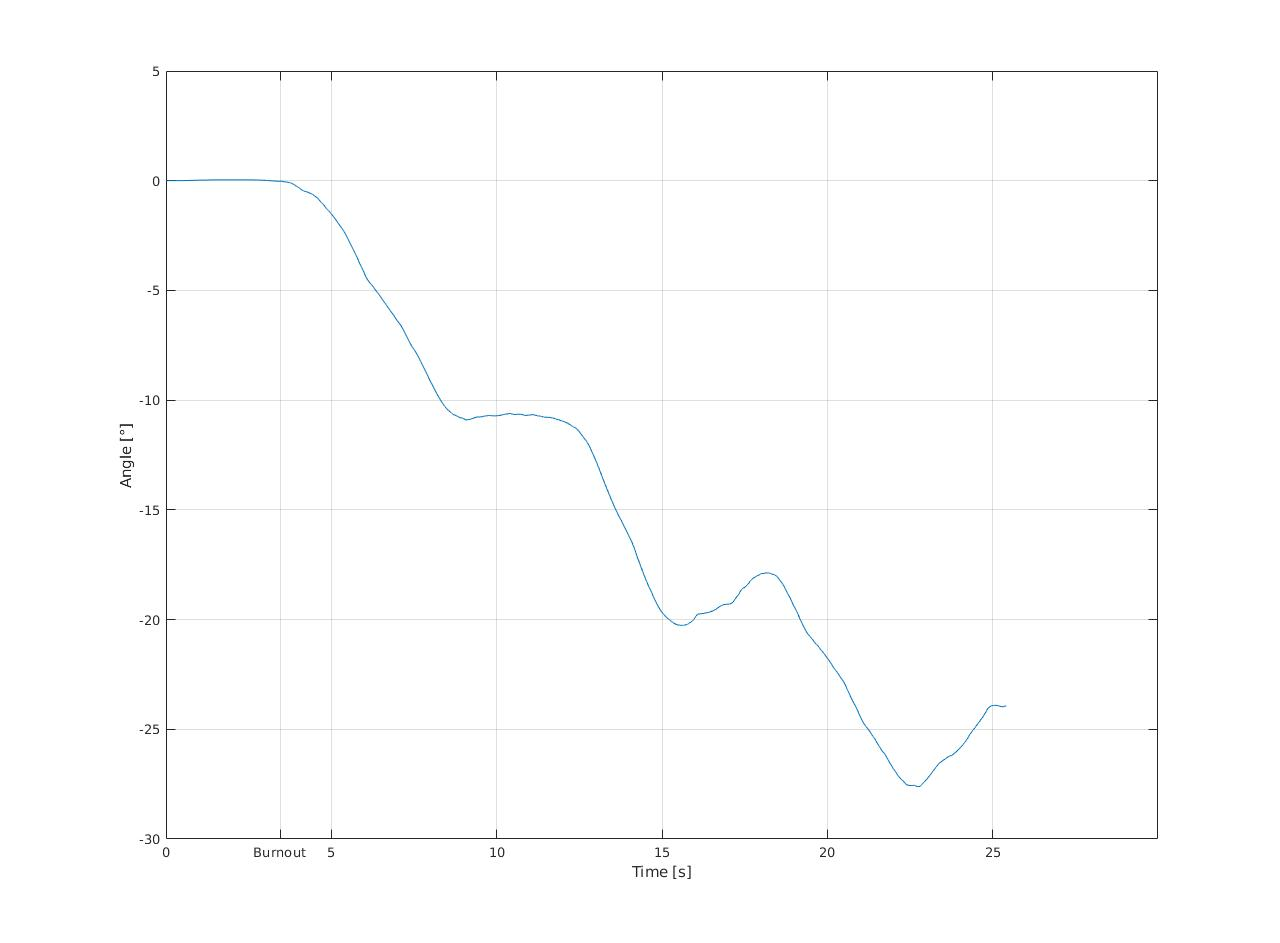
\includegraphics[width=.8\textwidth]{./Pictures/PitchAnglePlot.jpg}
 % PitchAnglePlot.jpg: 0x0 pixel, 300dpi, 0.00x0.00 cm, bb=
 \caption{Plot of pitch angle}
 \label{fig:PitchAnglePlot}
\end{figure}
For example figure \ref{fig:PitchAnglePlot} which represent the pitch angel.
In the system models there are no influences on this state value except for the measurements.
So to describe the changes of the value which are observed with the measurements a system noise has to have an impact on the pitch angle.
As it can be seen in the plot the angle does not change in a great manner until the burnout so the system noise till the burnout should also be rather small.
After the burnout the angle changes a lot more but keeps changing in the same way so this would reassemble a greater noise as before the burnout 
but the noise should be more or less the same over time. \\

As a second attempt since the system noise describes the capability of the value to change over time independent from the dynamic system description 
it can also be achieved due deviating the ground truth value vector.
For this the following matlab code can be used.
\begin{lstlisting}[caption={System noise generation with deviation}]
ACEL = abs(diff(a));				% Deviating the gournd truth acceleration
ACEL = filter(ones(1,100)*1/100,1,ACEL);	% Low pass filtering
ACEL = [ACEL ACEL(end)];			% Maintain vector length
\end{lstlisting}
This shows that after the deviation the absolute value from those is taken since a variance cannot or should not be negative.
After that the values are low pass filtered to smooth out more steady system noise description.

\subsection{Sensor Outfall}

An additional interesting scenario which can be observed with the simulation is the outfall of sensors.
This is needed to test the reliability requirements which states that the algorithm should still be working (with less accuracy) if 2-3 sensor fail.
For this it has to be said that it has to be detected that a sensor fails to adjust the estimation algorithm.
If done so the variance can be adjusted for this sensor in the same way as stated above, by maxing its variance out.

It is achieved by a simple if statement which does exactly that if a sensor fail is recognised.

\subsection{Loop}
Finally the state estimation is implemented in a simple loop which iterates trough each given time stamp.
First the needed vectors and matrices have to be initialised with the right value.
In the most system model versions the u vector remains zero while all measurements are brought into the estimation loop trough the y vector.
In the others the acceleration and the pitch angle are brought into the estimation loop over the u vector an the remaining measurements trough the y vector.
Also the current state vector x has to be initialised with the value that those states have at the start, 
which is presumably zero for all states except pressure and temperature.\\
The loop itself calculates the equation as they were stated in chapter \ref{ch:Approach}.
In addition if values from the measurements can not be transformed into the state vector values directly or with a linear calculation,
they have to be transformed first before entering the system.
For example pressure and temperature into height or acceleration and pitch angle into pure vertical acceleration.\\
Below is an example for the estimation loop for a rank five system.
It contains height, speed, acceleration, acceleration offset and pitch angle as state variables.
\begin{lstlisting}[caption={State Estimation Loop}]
% Initalzation
u = zeros(1,length(TimeVec));                       %Input vector is zero
y = [h_mes_GPS;a_mes;p_mes_1;p_mes_2;phi_mes];      %Output are the measurements
x = [0;0;0;0;0];                                    %Start Vector should be like this
P = eye(5);                                         %Standart can maybe be increased
Height1 = 0;
Height2 = 0;
Temp = T(1);

% Estimation loop
x_est_loop = zeros(size(x,1),length(TimeVec));     %Vector for the SE values
for k = 1:length(TimeVec)
    K = P*C'*pinv(C*P*C' + R_dyn_m(:,:,k));
    Height1 = CalcHeight(Po,p_mes_1(k),Temp,0,true,TgradSimu);
    Height2 = CalcHeight(Po,p_mes_2(k),Temp,0,true,TgradSimu);
    acc = a_mes(k) * cos(x(5)*pi/180);
    x = x + K*([h_mes_GPS(k);acc;Height1;Height2;phi_mes(k)] - C*x);
    P = (eye(5)-K*C)*P;
    
    x_est_loop(:,k) = x;                           %Save data from the Sensor fusion
    
    x = Ad*x + Bd*u(k);
    P = Ad*P*Ad' + Gd*Q_dyn_m(:,:,k)*Gd';

end
\end{lstlisting}



\chapter{Tests}
\label{ch:Tests}
In this chapter the test results of the tests that were taken to gain insight of the different system models and their performances are discussed.
First a general analysis is made by plotting the whole estimated flight as well a table which displays the errors of the different estimated values which were taken from multiple simulation cycles.
For this all estimations have been made with a mean acceleration offset of $ -1.31 m/s^2$  which was taken out of measurements from a test flight.
Also for the general analysis a perfectly linear temperature gradient of $-0.0065 °/m$ was used.
After that the different problematic properties of each system model is discussed in detail.
At the end the best system from the first tests has been further tested under different circumstances.


\section{Point Mass}
The first system model to test was the simple point mass model as described in chapter \ref{ch:Approach}.
While this implementation is a simple version it does already work surprisingly good.
In Figure \ref{fig:PointMassPerformance} the overall performance of its estimation of the different values can be seen.


\begin{figure}[h!]
 \centering
 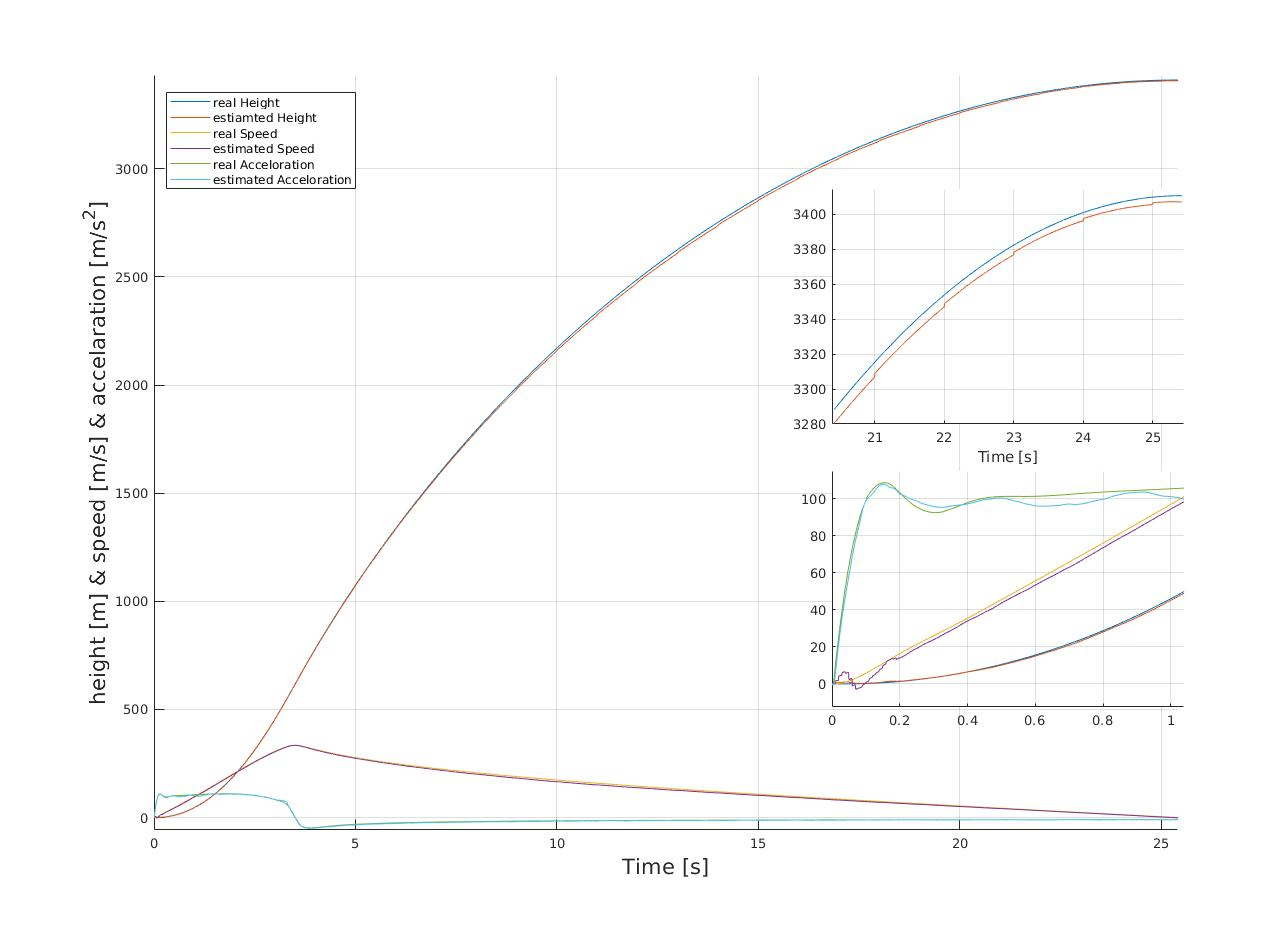
\includegraphics[width=.8\textwidth]{./Pictures/PointMassPerformance.jpg}
 % PointMassPerformance.jpg: 0x0 pixel, 300dpi, 0.00x0.00 cm, bb=
 \caption{The performance of the point mass system model over time}
 \label{fig:PointMassPerformance}
\end{figure}

Especially the first second (lower right corner) and the last five seconds (upper right corner) are interesting.
It can be seen that the system does not really have a settling time at all,
because the height is estimated at the minimal error at the beginning of the estimation.
On the other hand the speed needs around 0.2 seconds to settle on the right value.
Also a clear error on the estimation of the error can be seen after the speed has settled,
this is due to the fact that the estimator can trust the GPS and pressure measurements much more at the beginning than the acceleration measurements.
Therefore the estimator does adapt the acceleration estimation on the height and speed estimation at the start and not the other way around.
In the last five second it can be seen that the height is far more off as it was at the start.
Also the steps the estimation makes there are coming from the GPS measurements.
In addition Table \ref{tab:ErrorPointMass} shows the maximum, minimum, mean and median error of the estimated values.

\begin{table}[h!]
\centering
\begin{tabular}{cccccc}
\hline
\multicolumn{1}{|c|}{State Variable} & \multicolumn{1}{c|}{Unit} & \multicolumn{1}{c|}{Max} & \multicolumn{1}{c|}{Min} & \multicolumn{1}{c|}{Mean} & \multicolumn{1}{c|}{Median} \\ \hline
Height                            & $m$                         & 20.05                  & 1.18e-05                 & 4.72                    & 2.20                      \\
Speed                             & $m/s$                       & 3.42e+03               & 0                        & 3.40                    & 2.43                      \\
Acceleration                       & $m/s^2$   			& 17.79                  & 2.55e-05                 & 1.67                    & 1.55
\end{tabular}
\caption{Error of estimated state variables}
\label{tab:ErrorPointMass}
\end{table}

The most interesting value is the median from the height error because it is free from outliers.
It shows that the height error is with 2.2 meter slightly above the aimed 2 meter.
The 20 meter maximum error occurs around second 15 of the flight just before a new GPS measurement comes in.
At this time stamp the offset on the acceleration measurements does have a greater impact because the real value is in comparison to the start rather small.
In addition the height does change more between two GPS measurements than it does at the end of the flight, therefore greater errors in the interpolation between can occur.
Additionaly the minimum speed error occurs at the beginning of the estimation loop where the speed still zero.


\subsection{Greater Offset}
It has to be said that this only works while no sensor has a bigger offset.
Therefore these values come at the cost that they are not that trustworthy,
because the system noise on the acceleration has to be set to a greater value to get those good estimations.
An additional factor is also the pitch angle which does hinder this estimation if it changes in a great manner.
This can be seen in Figure \ref{fig:PointMassErrorWithOffset} which shows the state estimation error with different offsets.

\begin{figure}[h!]
 \centering
 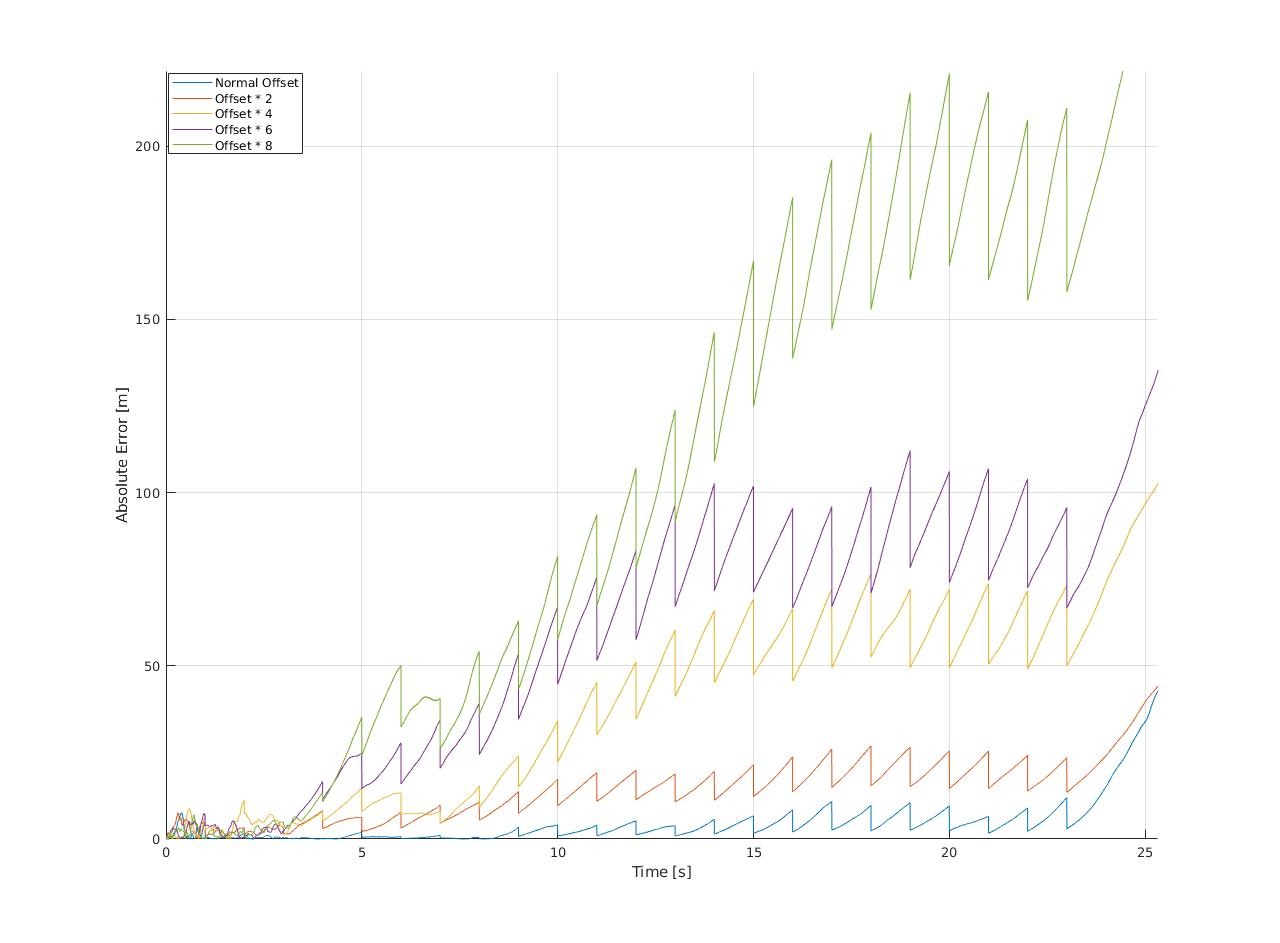
\includegraphics[width=.8\textwidth]{./Pictures/PointMassErrorWithOffset.jpg}
 % PointMassErrorWithOffset.jpg: 0x0 pixel, 300dpi, 0.00x0.00 cm, bb=
 \caption{Error during flight time with different offsets}
 \label{fig:PointMassErrorWithOffset}
\end{figure}


Table \ref{tab:PointMassPerformanceWithOffset} shows the mean and median of the error in the height depending on the offset on the accelerometer.

\begin{table}[h!]
\centering
\begin{tabular}{ccc}
\hline
\multicolumn{1}{|c|}{Offset} & \multicolumn{1}{|c|}{Mean}& \multicolumn{1}{|c|}{Median} \\ \hline
%
% & Mean & Median\\
Normal & 4.57 & 2.80\\
2 Times & 13.97 & 14.66\\
4 Times & 39.31 & 46.99\\
6 Times & 59.35 & 71.90\\
8 Times & 107.21 & 102.15
\end{tabular}
\caption{Error of the height in meter with changing offset}
\label{tab:PointMassPerformanceWithOffset}
\end{table}

This shows that the error which the estimator makes does rise exponentially.
So this is an issue which should be assessed by including an acceleration offset in the state vector.


\newpage
\section{Point Mass with Acceleration Offset}
The overall performance of this system model can be seen in the figure \ref{fig:PointMassOffsetPerformance}.

\begin{figure}[h!]
 \centering
 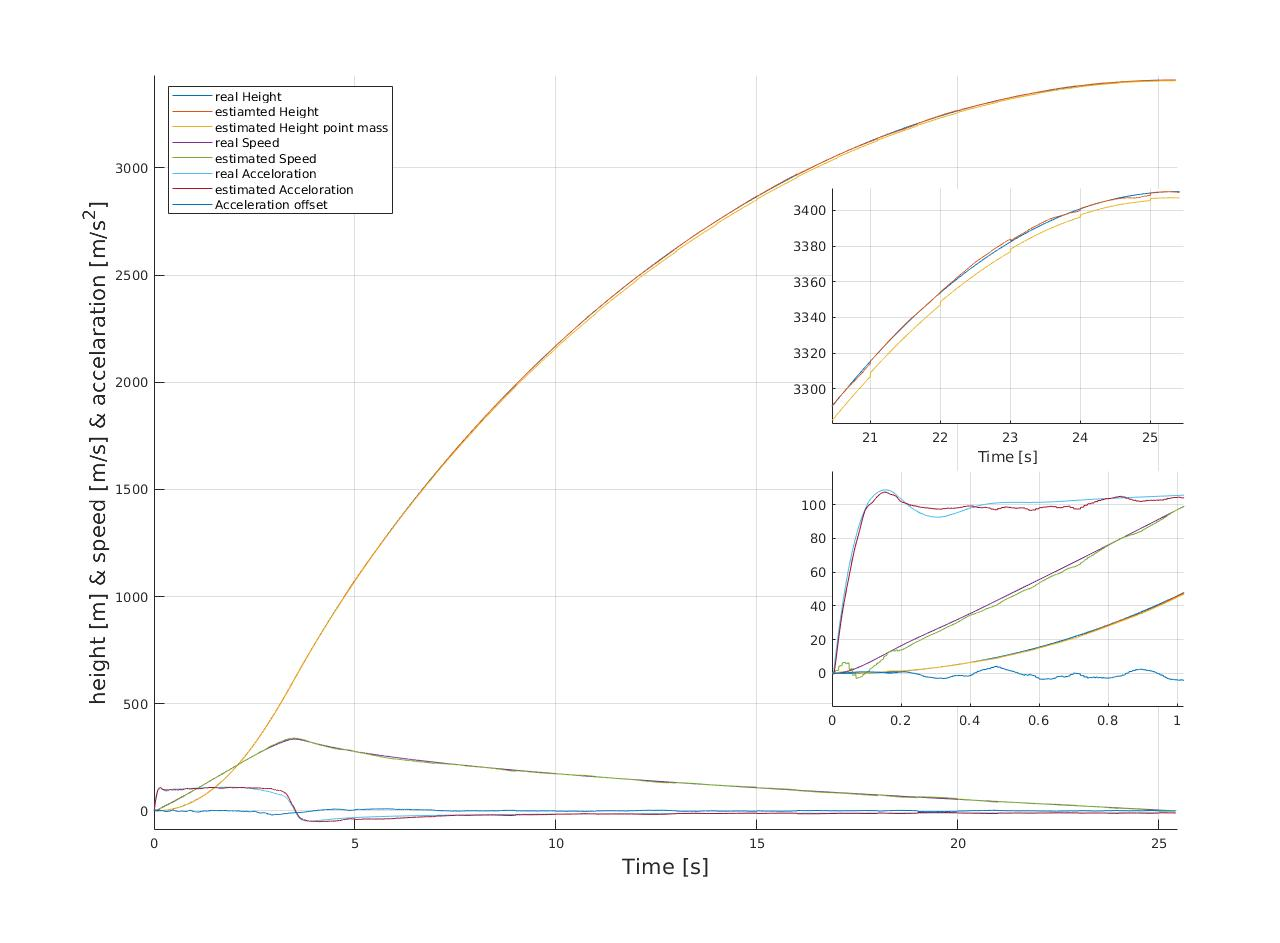
\includegraphics[width=.8 \textwidth]{./Pictures/PointMassOffsetPerformance.jpg}
 % PointMassOffsetPerformance.jpg: 0x0 pixel, 300dpi, 0.00x0.00 cm, bb=
 \caption{Performance of point mass with acceleration offset over time}
 \label{fig:PointMassOffsetPerformance}
\end{figure}

While the speed and height of it performs more or less the same way at the first second like the point mass system model,
a clear difference in the estimated acceleration can be seen.
This is possible due to the fact that the estimator can describe the difference in the system description between the speed and acceleration as the acceleration offset.
These dependencies can be seen after the settling of the speed where the estimator starts to change the acceleration offset value to adjust the acceleration.
The great advantage of this can be seen in the plot of the last five seconds of the height estimation (upper right plot).
Due to the better estimation of the acceleration over the whole time, the dependencies of the height on the acceleration is much more trustworthy.
When the rocket does rise at further height and the measurements of the barometers lose their accuracy,
the better acceleration measurements can be used to interpolate between the good GPS measurements.
This results in a much better height estimation at greater height.

\begin{table}[h!]
\centering
\begin{tabular}{cccccc}
\hline
\multicolumn{1}{|c|}{State Variable} & \multicolumn{1}{c|}{Unit} & \multicolumn{1}{c|}{Max} & \multicolumn{1}{c|}{Min} & \multicolumn{1}{c|}{Mean} & \multicolumn{1}{c|}{Median} \\ \hline
Height                            & $m$                         & 9.78                   & 2.98e-06                 & 1.33                    & 0.83                      \\
Speed                             & $m/s$                       & 78.79                  & 0                        & 3.18                    & 2.22                      \\
Acceleration                       & $m/s^2$   			& 165.87                  & 1.35e-05                 & 4.52                    & 2.64                     \\
Acceleration Offset                & $m/s^2$   			& 167.46                  & 2.66e-05                 & 4.44                    & 2.61
\end{tabular}
\caption{Error of estimated state variables point mass with acceleration offset}
\label{tab:ErrorPointMassAccelerationOffset}
\end{table}

Table \ref{tab:ErrorPointMassAccelerationOffset} shows the estimation errors of this model.
The entries that draw the attention are the maximum of the estimation errors from the acceleration and speed which is bigger than that of of the point mass system model.
These occurred due to one complete false estimation during one of the simulation and should not be seen as normal.
The interesting thing about this is that despite those big maxima, the mean value of the estimated height and speed are still better than the ones from the point mass system model.
Also can be seen that the median of the height error is just 0.83 meter. \\

As with the point mass system model Figure \ref{fig:PointMassOffsetErrorWithOffset} shows the error during a flight with different sensor offsets.
It can clearly be seen that while the mean error does rise by some value, it always gets back to zero and therefore overall this system preforms better as the simple point mass.

\begin{figure}[h!]
 \centering
 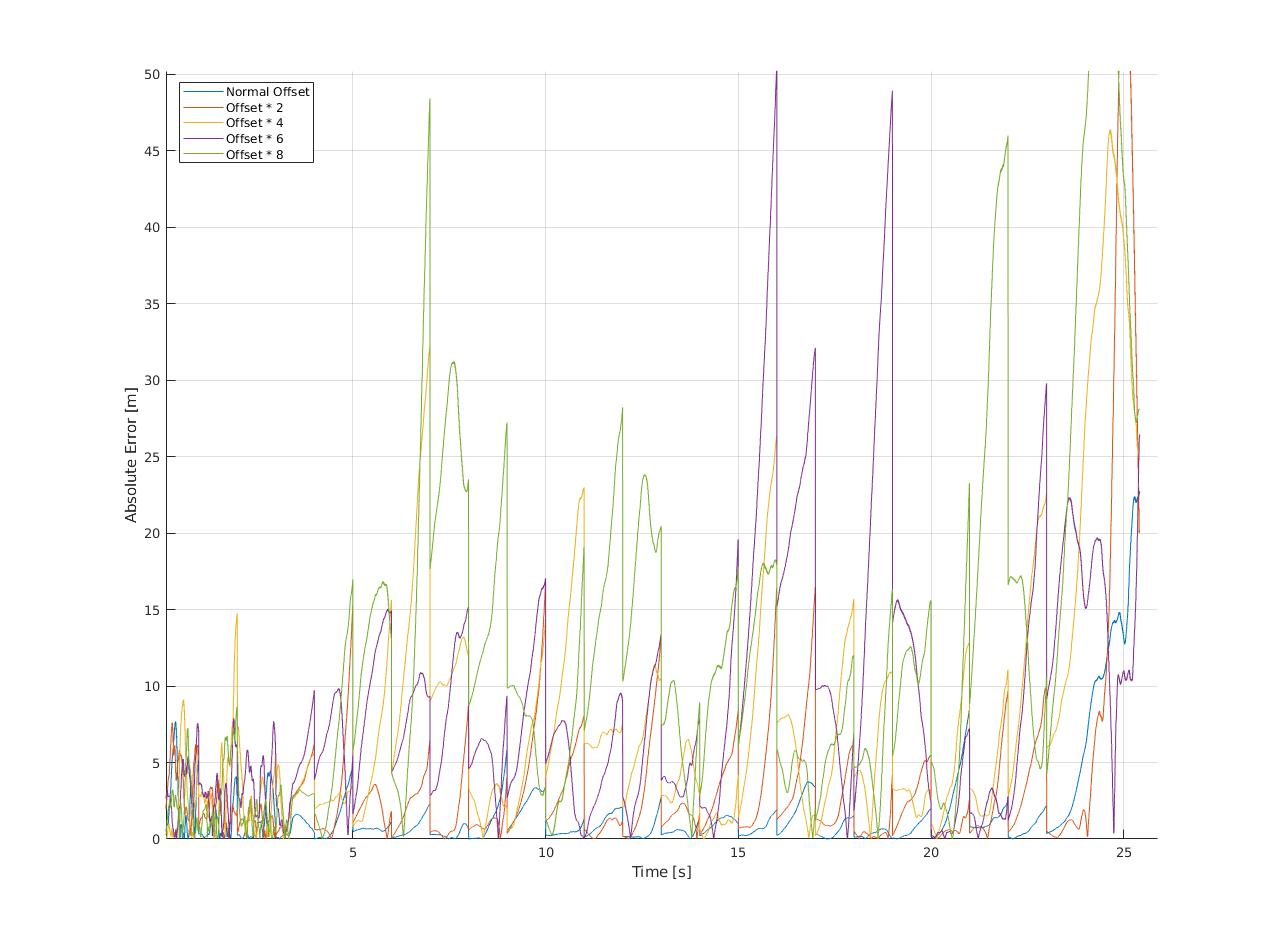
\includegraphics[width=0.8\textwidth]{./Pictures/PointMassOffsetErrorWithOffset.jpg}
 % PointMassOffsetErrorWithOffset.jpg: 0x0 pixel, 300dpi, 0.00x0.00 cm, bb=
  \caption{Error during flight time with different offsets}
 \label{fig:PointMassOffsetErrorWithOffset}
\end{figure}


\newpage
\section{Point Mass with Pressure}
As with the ones above the overall performance of the system model which uses the pressure as an additional state variable can be seen in Figure \ref{fig:PointMassPressurePerformance}.

\begin{figure}[h!]
 \centering
 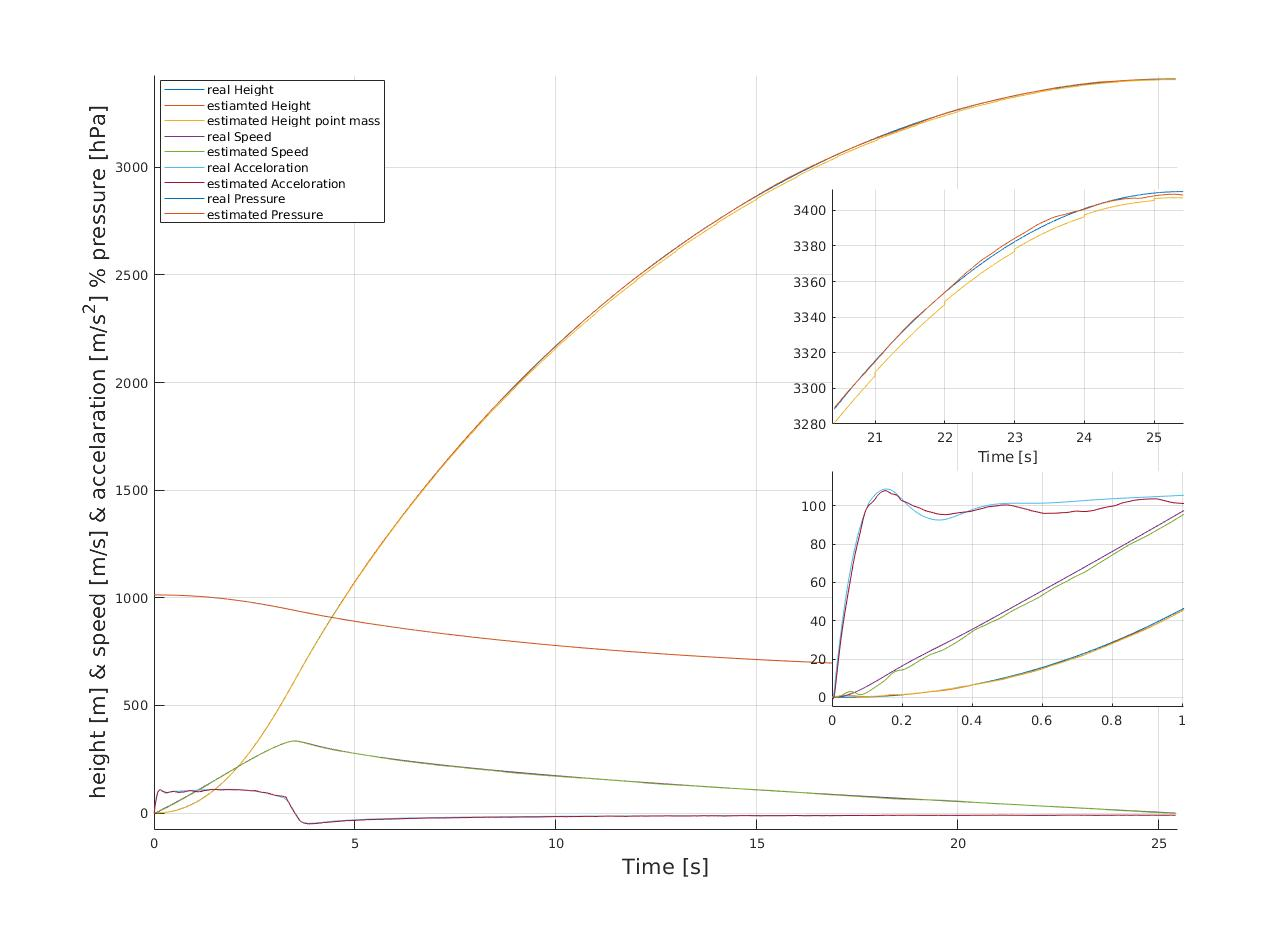
\includegraphics[width=.8 \textwidth]{./Pictures/PointMassPressurePerformance.jpg}
 % PointMassOffsetPerformance.jpg: 0x0 pixel, 300dpi, 0.00x0.00 cm, bb=
 \caption{Performance of point mass with pressure over time}
 \label{fig:PointMassPressurePerformance}
\end{figure}

This shows that it performs as good as a system which uses acceleration offset as a state value.
It can be seen that the pressure is so well estimated that it fully covers the real pressure curve in the plot.
Also in the plot of the first second it can be seen that there is no settling time for either of the estimation values.
The height in the last 5 second shows too that the impact from the GPS measurements are much smaller than in the first model (no staircase like adjustments of the height as seen in the point mass system model).

\begin{table}[h!]
\centering
\begin{tabular}{cccccc}
\hline
\multicolumn{1}{|c|}{State Variable} & \multicolumn{1}{c|}{Unit} & \multicolumn{1}{c|}{Max} & \multicolumn{1}{c|}{Min} & \multicolumn{1}{c|}{Mean} & \multicolumn{1}{c|}{Median} \\ \hline
Height                            & $m$                         & 5.16                   & 1.47e-06                 & 1.20                    & 0.96                      \\
Speed                             & $m/s$                       & 8.80                   & 0                        & 1.89                    & 1.61                      \\
Acceleration                      & $m/s^2$   			& 18.14                  & 3.90e-05                 & 1.80                    & 1.63                      \\
Pressure                  	  & $hPa$   			& 0.72                   & 4.69e-06                 & 0.13                    & 0.11
\end{tabular}
\caption{Error of estimated state variables point mass with pressure}
\label{tab:ErrorPointMassPressure}
\end{table}

Like above Table \ref{tab:ErrorPointMassPressure} shows the error over the simulations.
The error on the height is nearly as good as with the acceleration offset, while the maxima of the differences are quite smaller than above.
These results therefore have much better mean values of the errors.

\subsection{Wrong Temperature Gradient}
While it does increase the accuracy it does also increase the needed computational effort due to the fact that to get a real added value from this,
the height out of the pressure has to be calculated at each time step with the help of the estimated pressure.
In addition when the temperature gradient is chosen wrong it deeply affects the estimation as can be seen in Figure \ref{fig:PointMassVSPressure}.
The errors there were low pass filtered with a moving average filter for better visualisation.

\begin{figure}[h!]
 \centering
 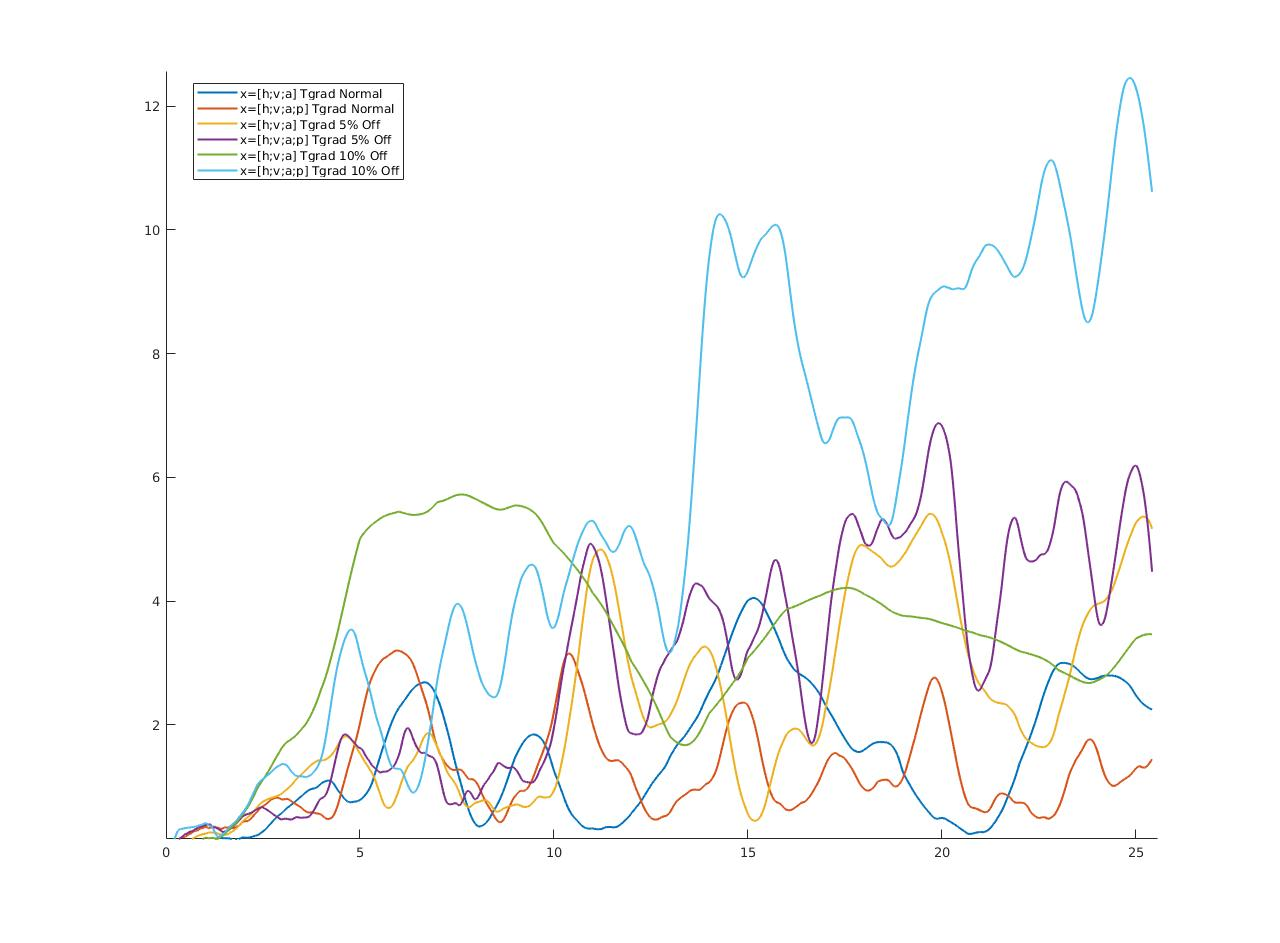
\includegraphics[width=.8 \textwidth]{./Pictures/PointMassVSPressure.jpg}
 % PointMassVSPressure.jpg: 0x0 pixel, 300dpi, 0.00x0.00 cm, bb=
 \caption{Plot of point mass vs the pressure low pass filtered}
 \label{fig:PointMassVSPressure}
\end{figure}

In this figure the error for both, a system with acceleration offset (which therefore can depend more on the accelerometer measurements)
and a system model with the pressure in the state vector are compared against each other.
While they preform equaly good as long as the temperature gradient is determined correctly,
if the gradient is determined wrong by just 5 percent it already performs less accurate than all of the other tested system models.
This is a problem due to the fact that the temperature gradient will most certainly not be correct during the whole flight.
With this it can be seen that the overall system performance of this model is more or less the same as with the normal point mass system.
On the other hand if the error on the temperature gradient is exactly known, the noise onto those measurements can be adjusted which
results in a gain of robustness for the whole estimation.

To summarize it, the pressure as a state variable is a risky but if done right a helpful adjustment of the system model.

\newpage
\section{Point Mass with Pitch angle}
The pitch angle is difficult to estimate because it has no measured dependencies on its own.
Therefore the Kalman filter does just something like a real time low pass filtering on those measurements.
This can be seen in Figure \ref{fig:PointMassPitchAnglePerformance}. The estimated pitch angle there changes slower than the generated measurements value which can be seen in chapter \ref{ch:Implementation}.

\begin{figure}[h!]
 \centering
 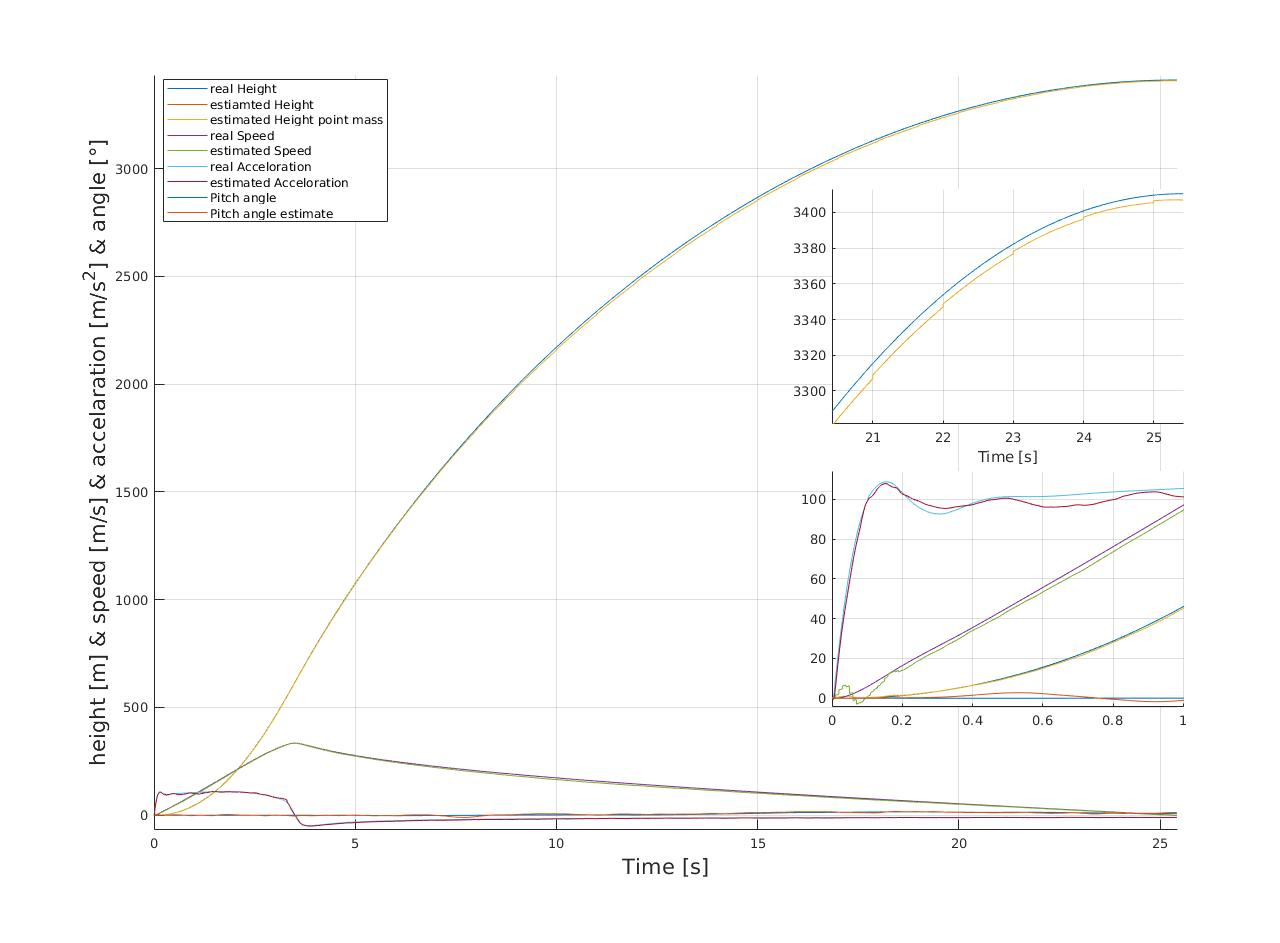
\includegraphics[width=.8 \textwidth]{./Pictures/PointMassPitchAnglePerformance.jpg}
 % PointMassOffsetPerformance.jpg: 0x0 pixel, 300dpi, 0.00x0.00 cm, bb=
 \caption{Performance of point mass with pitch angle over time}
 \label{fig:PointMassPitchAnglePerformance}
\end{figure}

The overall performance is more or less the same than that of the normal point mass system. This can espacially be seen in the last five seconds of the height estimation where both estimations are equal to each other (the estimation of the point mass system model does overlap the one of the system model which includes the pitch angle estimation).
The one big difference which can be seen in the plot of the first second is that the estimator tries to correct the wrong acceleration measurements (due to the offset) with the change of the pitch angle.
But because the system noise on the pitch angle states that it does not change in a great manner until the burnout the influence is restricted.

\begin{table}[h!]
\centering
\begin{tabular}{cccccc}
\hline
\multicolumn{1}{|c|}{State Variable} & \multicolumn{1}{c|}{Unit} & \multicolumn{1}{c|}{Max} & \multicolumn{1}{c|}{Min} & \multicolumn{1}{c|}{Mean} & \multicolumn{1}{c|}{Median} \\ \hline
Height                            & $m$                         & 20.24                  & 4.46e-06                 & 4.75                    & 2.24                      \\
Speed                             & $m/s$                       & 78.57                   & 0                        & 3.42                   & 2.44                      \\
Acceleration                      & $m/s^2$   			& 17.79                  & 6.26e-05                 & 1.68                    & 1.55                      \\
Angle	                  	  & $°$   			& 12.26                   & 2.46e-05                 & 2.41                  & 1.90
\end{tabular}
\caption{Error of estimated state variables point mass with pressure}
\label{tab:ErrorPointMassPitchAngle}
\end{table}

In Table \ref{tab:ErrorPointMassPitchAngle} the errors of the estimation can be seen once again.
It shows that the values are nearly the same as the ones from the point mass system.

\subsection{Small Influence}
This results in the conclusion that the influence of the pitch angle is much smaller than thought.
This mainly because the pitch angle does only start to get to a greater value after the burnout.
After this the vertical acceleration is much smaller and therefore an error of the angle by a few degrees does not have a big impact.
In other words for example if the real angle is 10 degrees, the measurement at this point is around 18 degrees while the estimation is 11 degrees.
Then this means the measured acceleration of for example 10.15$m/s^2$ should be corrected to 10$m/s^2$. With the estimated angle it is corrected to 9.97$m/s^2$,
while with the measured angle it is corrected to 9.66$m/s^2$. So for this example an error of 8 degrees would only result in a false estimation of 0.31$m/s^2$.
Although this error does not develop in a linear fashion especially when the angle has a greater value, due to the rather small accelerations after the burnout the impact of the noisy measurements is still strongly limited.
This can be seen in the plot on Figure \ref{fig:PointMassVSPitch} where the estimation which uses the pitch angle as an additional state variable makes the performance just slightly better.
\begin{figure}[h!]
 \centering
 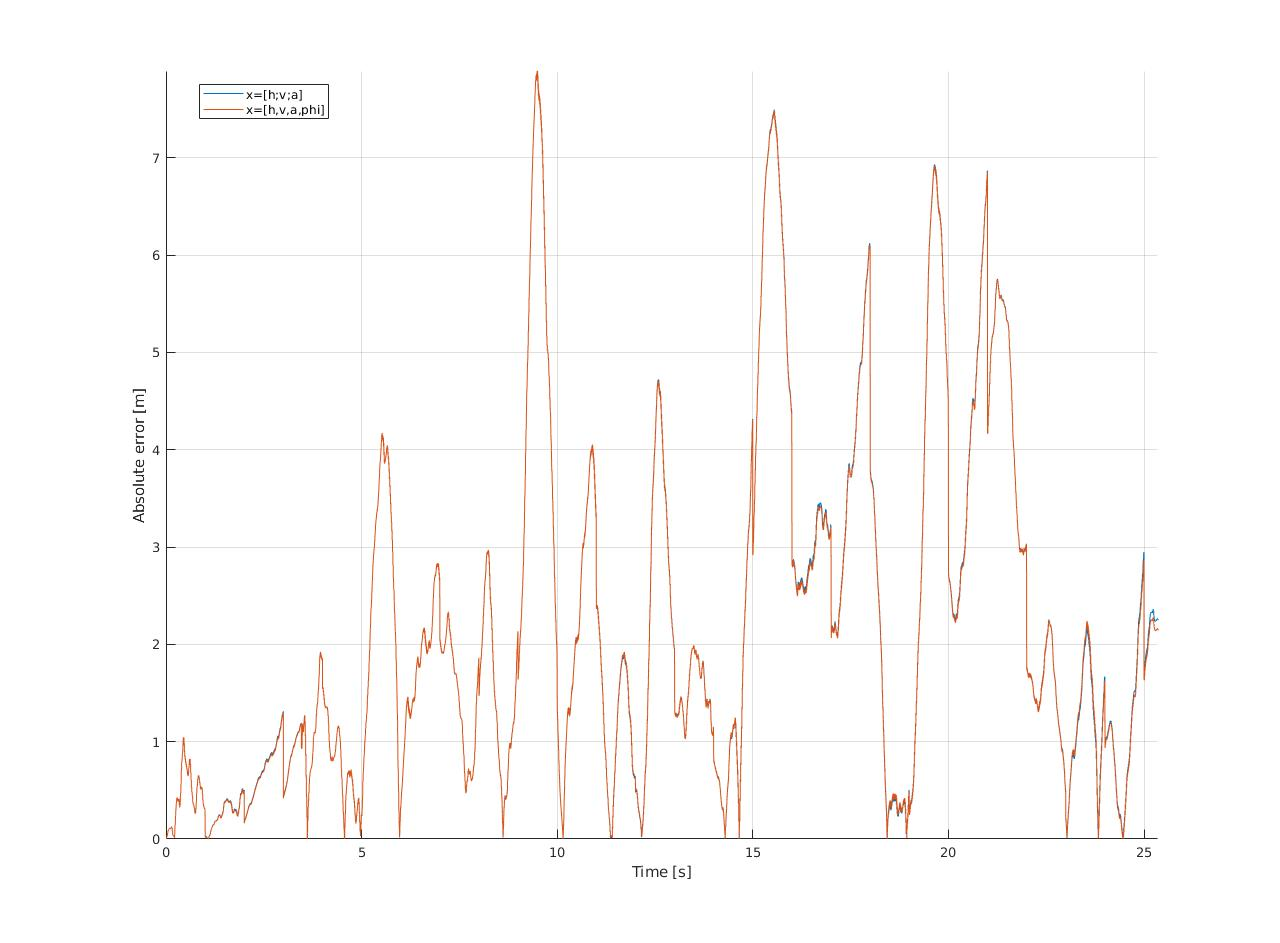
\includegraphics[width=.8 \textwidth]{./Pictures/PointMassVSPitch.jpg}
 % PointMassVSPitch.jpg: 0x0 pixel, 300dpi, 0.00x0.00 cm, bb=
 \caption{Estimation error over time from point mass system with and without pitch angle inclusion}
 \label{fig:PointMassVSPitch}
\end{figure}

\newpage
\section{Point Mass with Acceleration as input}
The overall performance of this system model is shown in Figure \ref{fig:PointMassAccInputPerformance}.

\begin{figure}[h!]
 \centering
 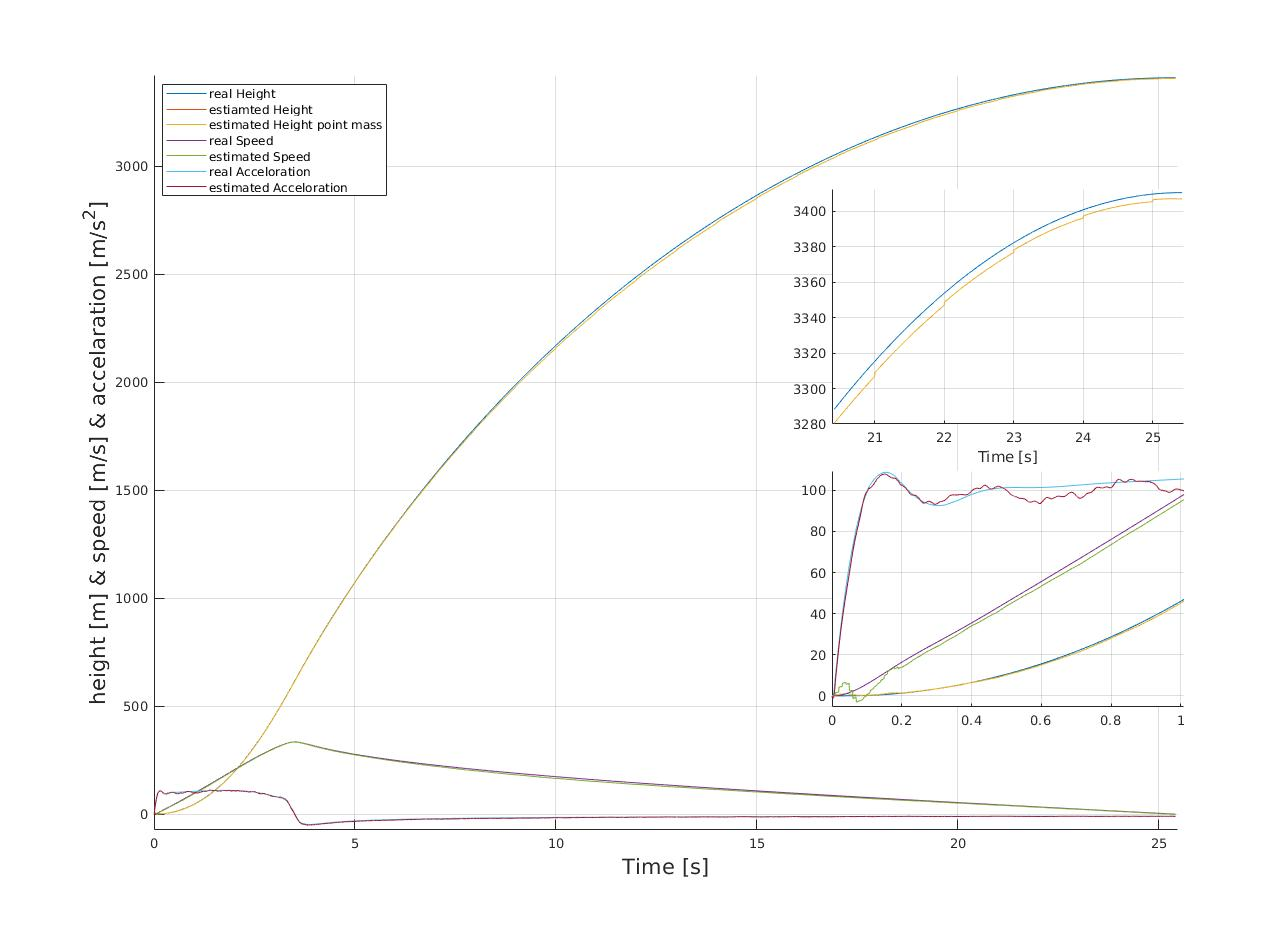
\includegraphics[width=.8 \textwidth]{./Pictures/PointMassAccInputPerformance.jpg}
 % PointMassOffsetPerformance.jpg: 0x0 pixel, 300dpi, 0.00x0.00 cm, bb=
 \caption{Performance of point mass with acceleration as input over time}
 \label{fig:PointMassAccInputPerformance}
\end{figure}

Its performance does also resemble the point mass system model quite well but without any significant improvement.
As above with the pitch angle the estimated height of both systems do overlap over more or less the whole flight.
This can be seen in the upper right corner of Figure \ref{fig:PointMassAccInputPerformance} where due to the overlap only the values from the point mass system model is visible.
The difference in the errors between this system model and the normal point mass model occurs more due to rounding errors of the simulation than due to really better estimation.
This can be concluded by fact that this system model performs sometimes slightly better and sometimes slightly worse than the point mass system, therefore there is no real gain in the implementation this way.

In addition the plot of the first second of the estimation shows that the acceleration estimation has more noise on it than in the other system models.
This is because the acceleration has no model dependencies in this implementation, it is taken directly as system input.
With this the system noise on the acceleration has to resemble either the measurement or the system noise.
In this implementation it was used to bring the measurement noise into the system and therefore the low pass characteristics of the system noise is lost.
In other words with a measurement as input a tuning parameter (either system or measurement noise) which could compensate the corresponding state value cannot be used.
So there is no real gain in this implementation and it will therefore not be implemented in the final system model.

\begin{table}[h!]
\centering
\begin{tabular}{cccccc}
\hline
\multicolumn{1}{|c|}{State Variable} & \multicolumn{1}{c|}{Unit} & \multicolumn{1}{c|}{Max} & \multicolumn{1}{c|}{Min} & \multicolumn{1}{c|}{Mean} & \multicolumn{1}{c|}{Median} \\ \hline
Height                            & $m$                         & 20.05                  & 7.21e-06                 & 4.71                    & 2.18                      \\
Speed                             & $m/s$                       & 78.49                  & 0                        & 3.38                    & 2.40                      \\
Acceleration                       & $m/s^2$   			& 10.65                  & 0                        & 1.60                    & 1.43
\end{tabular}
\caption{Error of estimated state variables point mass with acceleration as input}
\label{tab:ErrorPointMassAccelerationInput}
\end{table}

\newpage
\section{Point Mass with offset and better calculated system noise}
The better calculated system noise for this estimation was calculated as stated in chapter \ref{ch:Implementation}.
This has been done by calculating the discrete system noise matrix Gd with the integration method as well as
derive the perfect measurements and then low pass filter them to get better system noise vectors.
This improvement had to be done on a system which uses the acceleration offset as well in the state vector to get the maximum possible gain out of this implementation.
This results in an overall system performance as seen in Figure \ref{fig:PointMassBetterNoisePerformance}

\begin{figure}[h!]
 \centering
 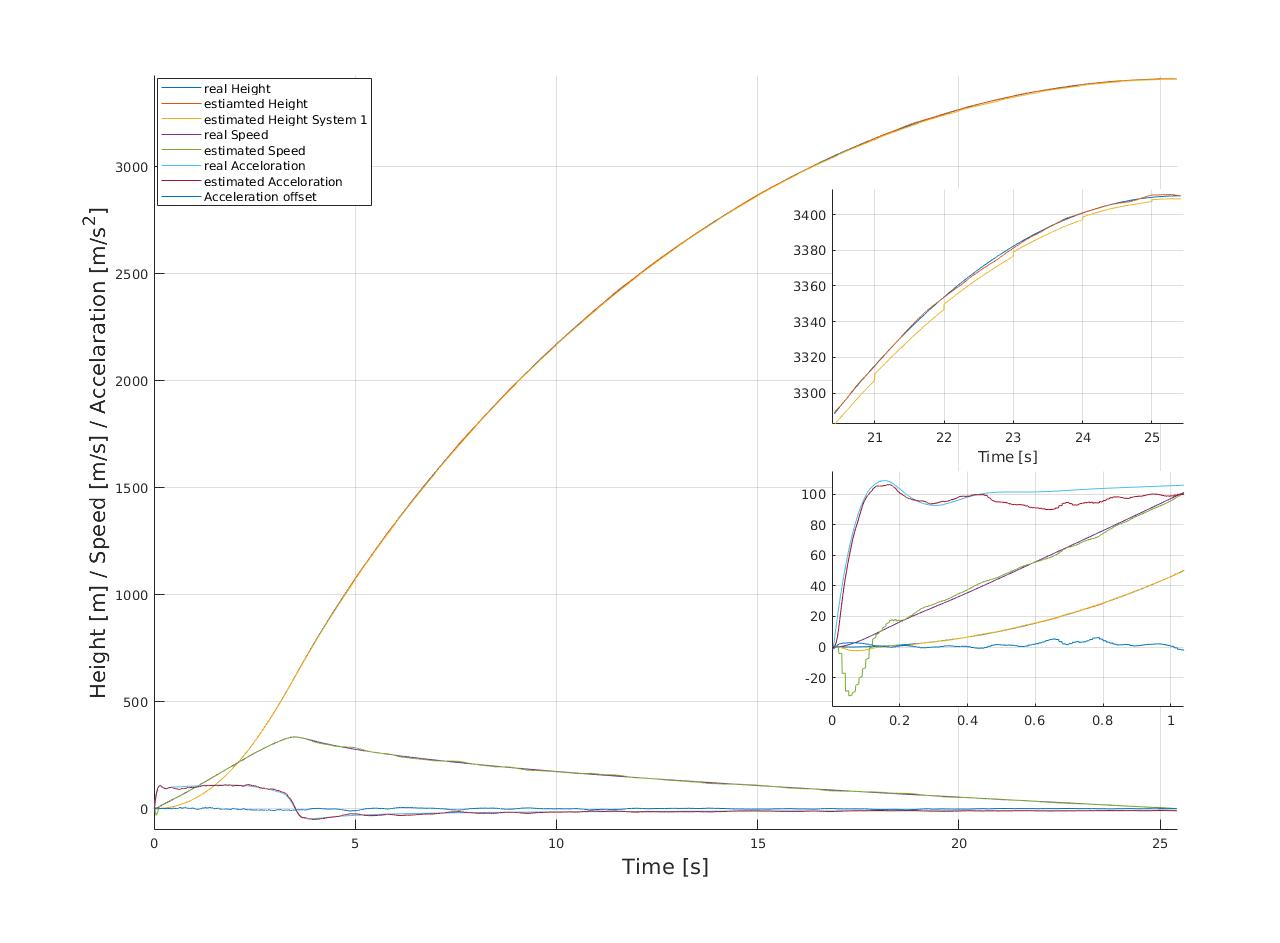
\includegraphics[width=.8 \textwidth]{./Pictures/PointMassBetterNoisePerformance.jpg}
 % PointMassOffsetPerformance.jpg: 0x0 pixel, 300dpi, 0.00x0.00 cm, bb=
 \caption{Performance of point mass with better system noise over time}
 \label{fig:PointMassBetterNoisePerformance}
\end{figure}

This system performs much like the one with acceleration offset as a state vector.
The greatest difference can be seen in the first half second where the acceleration is nearly perfectly estimated.
Also does the acceleration offset not change as much as in the system model without the improved system noise calculation.
This is because with the better system noise an optimal estimation can be achieved with less effort since the influence of the acceleration offset is more clearly defined.

\begin{table}[h!]
\centering
\begin{tabular}{cccccc}
\hline
\multicolumn{1}{|c|}{State Variable} & \multicolumn{1}{c|}{Unit} & \multicolumn{1}{c|}{Max} & \multicolumn{1}{c|}{Min} & \multicolumn{1}{c|}{Mean} & \multicolumn{1}{c|}{Median} \\ \hline
Height                            & $m$                         & 9.74	                  & 8.11e-06                 & 1.28                    & 0.73                      \\
Speed                             & $m/s$                       & 78.58                   & 0                        & 2.79                    & 1.85                      \\
Acceleration                       & $m/s^2$   			& 86.93                   & 4.07e-05                 & 3.57                    & 1.96                     \\
Acceleration Offset                & $m/s^2$   			& 88.60                   & 2.52e-05                 & 4.59                    & 2.59
\end{tabular}
\caption{Error of estimated state variables point mass with acceleration offset and better system noise}
\label{tab:ErrorPointMassBetterNoise}
\end{table}

Table \ref{tab:ErrorPointMassBetterNoise} shows that the system performs pure error wise better than each of the other system models discussed before.
While it also contains big maxima in speed, the acceleration and acceleration offset values are smaller than the ones of the system with only acceleration offset.
Due to that the mean values (except the offset) are still better than most other.

Figure \ref{fig:PointMassVSBetterNoise} shows that an overall better estimation can be achieved with this tactic.
\begin{figure}[h!]
 \centering
 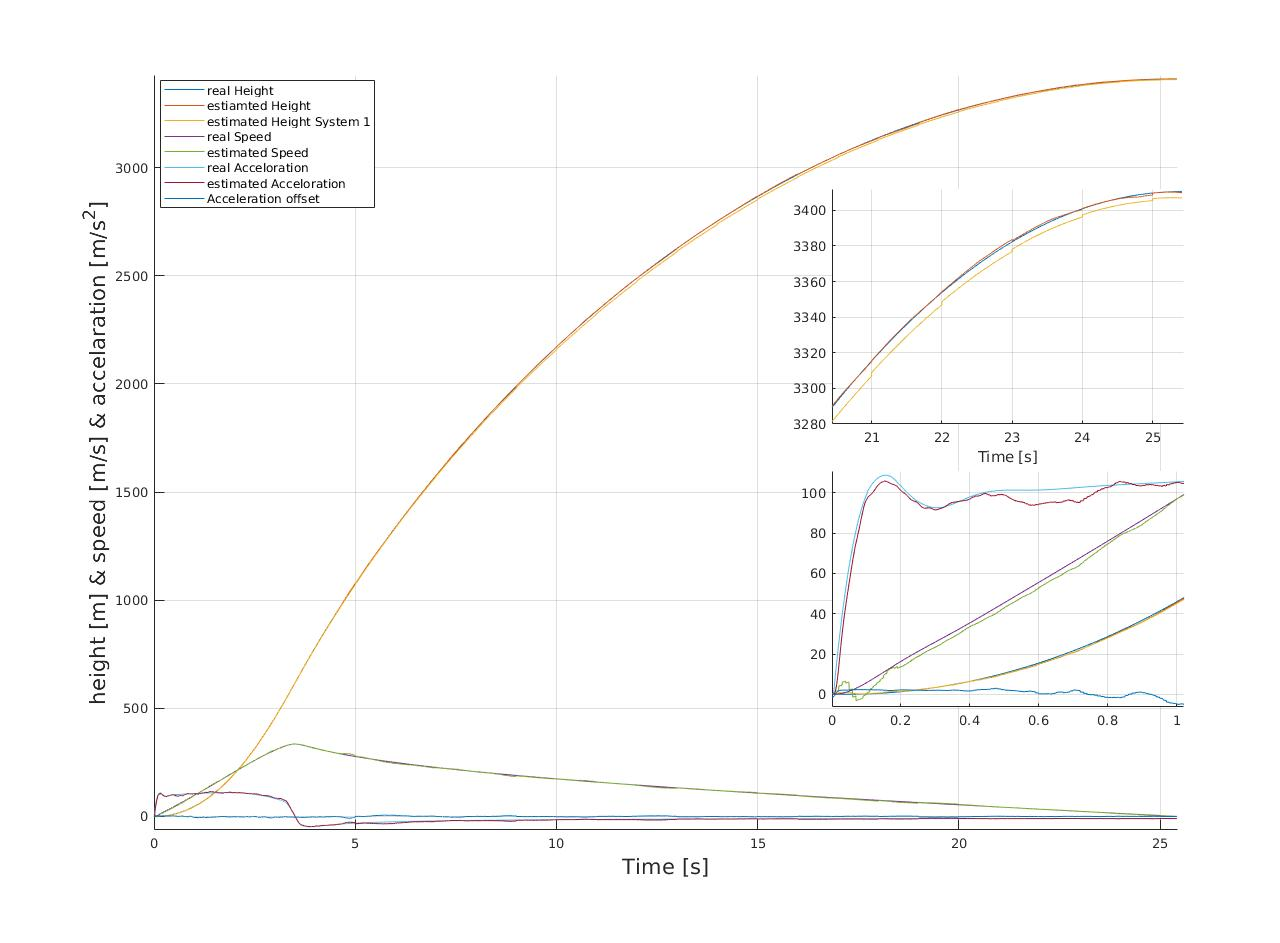
\includegraphics[width=.8\textwidth]{./Pictures/PointMassVSBetterNoise.jpg}
 % PointMassVSBetterNoise.jpg: 0x0 pixel, 300dpi, 0.00x0.00 cm, bb=
 \caption{Error over time with and without better system noise}
 \label{fig:PointMassVSBetterNoise}
\end{figure}
This is mostly due to the better system noise vector which can be much better estimated this way.
Also the additional effort to access this system model only occurs on the preparation,
while it does have no effect on the computational effort during the flight itself.
So this approach of the state estimation should be used any time if available.

\newpage
\section{With and without GPS}
It is not certain that the GPS will be working in the next competitions as already stated in the introduction.
In addition the GPS sensor data needs more time to be measured and can therefore arrive too late to be included correctly.
There is the possibility of back calculation to include such too late arrived measurements into the state estimation but this needs a lot of computational effort \cite{SimonDan2006Ose:}.

Because of this, the estimation without the GPS measurements are tested with a point mass system model to find its direct impacts.
Figure \ref{fig:PointMassWithWithoutGPS} shows the plot of different estimations with and without working GPS.

\begin{figure}[h!]
 \centering
 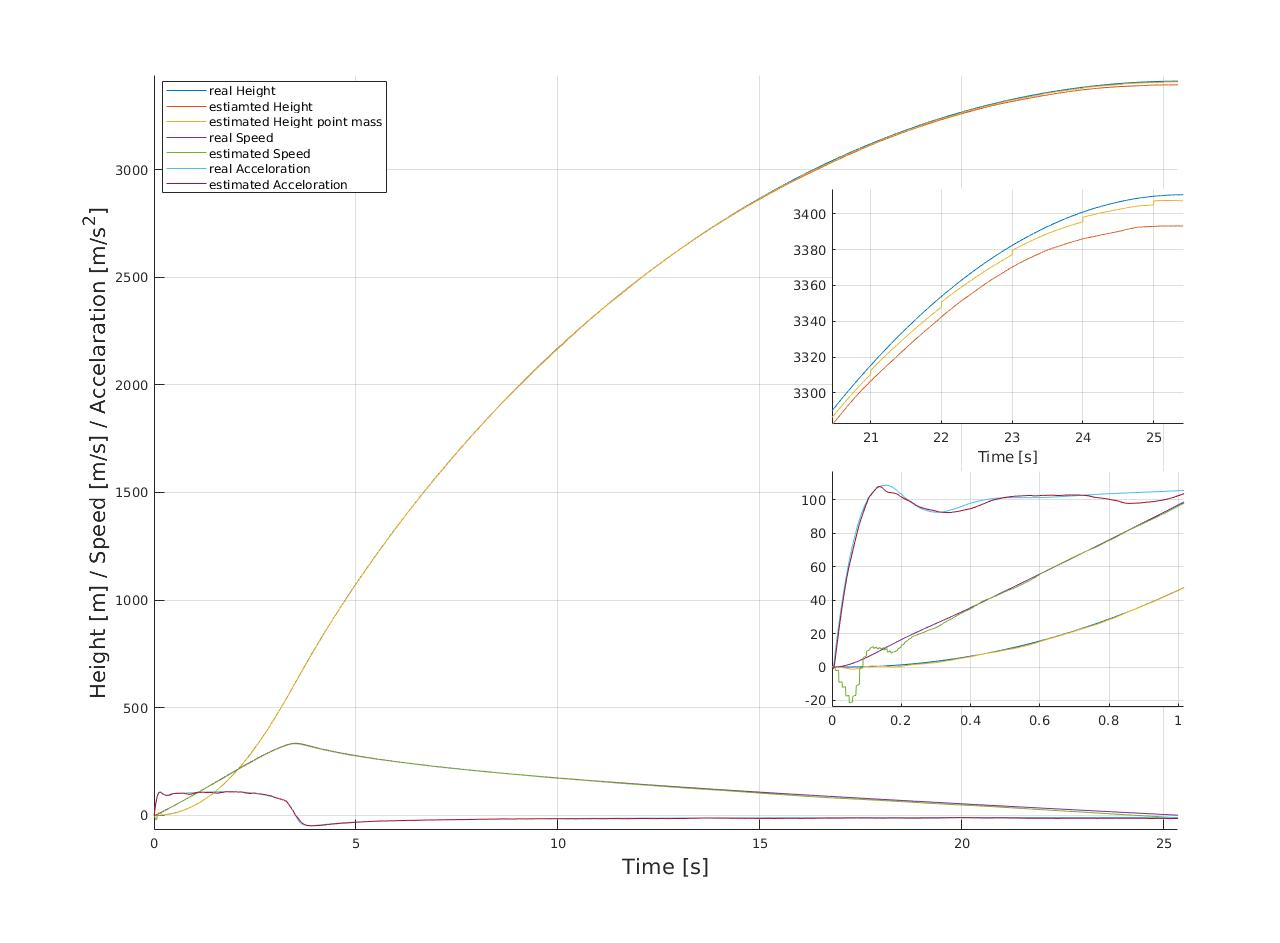
\includegraphics[width=.8 \textwidth]{./Pictures/PointMassWihtoutGPSPerformance.jpg}
 % PointMassOffsetPerformance.jpg: 0x0 pixel, 300dpi, 0.00x0.00 cm, bb=
 \caption{Performance of point mass without GPS over time}
 \label{fig:PointMassWithoutGPSPerformance}
\end{figure}

As expected the height is further away from the ground truth in the last five seconds plot than the one estimated with GPS measurements.
Also the staircase like correction steps which come from the GPS measurements are missing.
This behaviour was expected because the the GPS measurements are most important at great heights were the remaining measurements lose their credibility.


\begin{table}[h!]
\centering
\begin{tabular}{cccccc}
\hline
\multicolumn{1}{|c|}{State Variable} & \multicolumn{1}{c|}{Unit} & \multicolumn{1}{c|}{Max} & \multicolumn{1}{c|}{Min} & \multicolumn{1}{c|}{Mean} & \multicolumn{1}{c|}{Median} \\ \hline
Height                            & $m$                         & 31.20                  & 5.77e-05                 & 8.97                    & 5.20                      \\
Speed                             & $m/s$                       & 78.58                  & 0                        & 6.35                    & 4.86                      \\
Acceleration                       & $m/s^2$   			& 17.78                  & 7.60e-05                 & 3.48                    & 2.34
\end{tabular}
\caption{Error of estimated state variables point mass without GPS measurements}
\label{tab:ErrorPointMassWithoutGPS}
\end{table}

Table \ref{tab:ErrorPointMassWithoutGPS} which displays the errors from the estimations shows that as expected the error is bigger in each value.
Also the maximum height error of over 30 meter shows that the normal state estimator is really depending on the GPS measurements.

\subsection{Wrong temperature gradient}
This system has to depend strongly on the barometer measurements to calculate the height.
Therefore the problem of a wrong temperature gradient arises once again.
To show this the estimation results with different temperature gradients are plotted in Figure \ref{fig:PointMassWithWithoutGPS}.

\begin{figure}[h!]
 \centering
 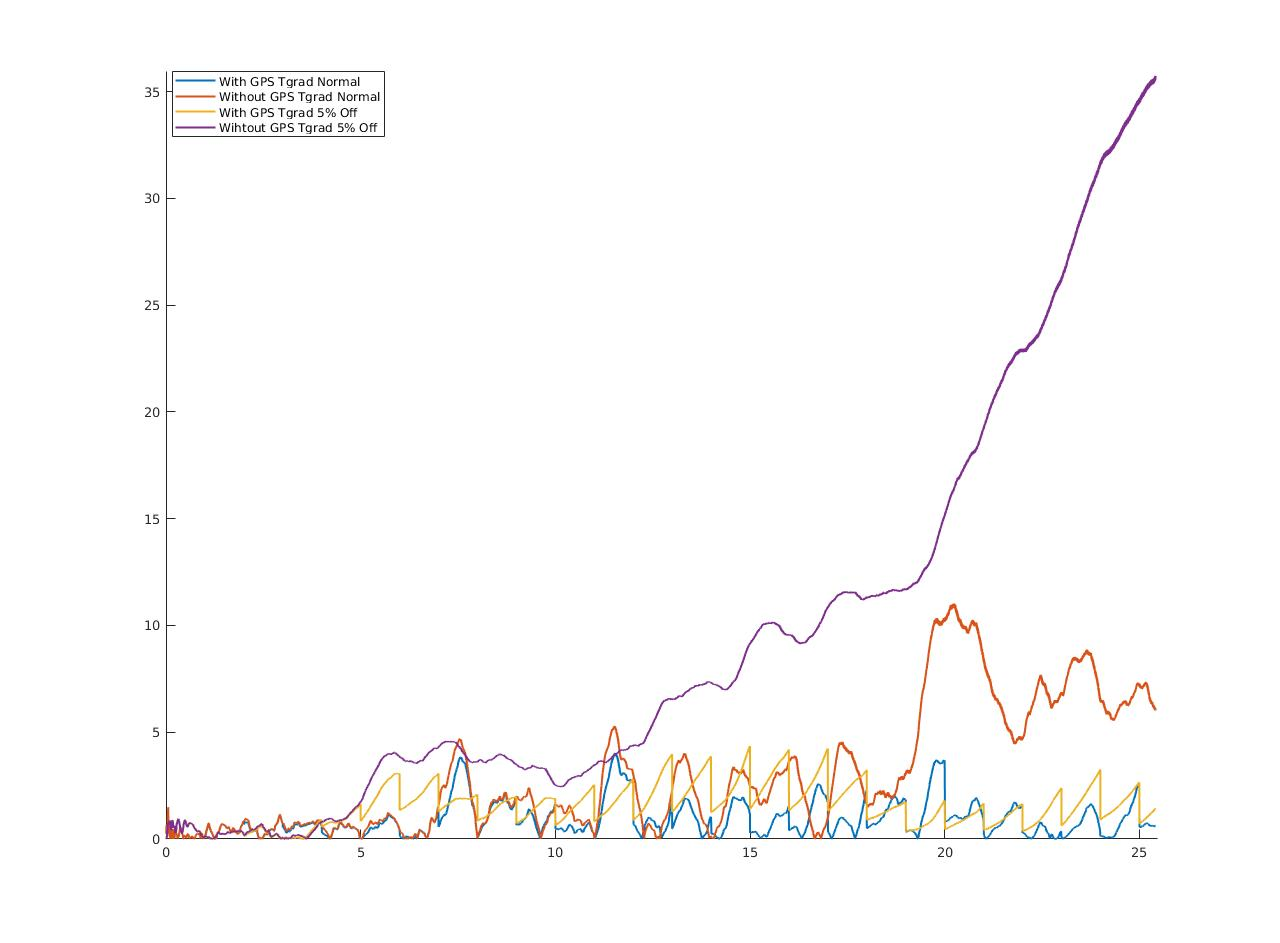
\includegraphics[width=.8\textwidth]{./Pictures/PointMassWithWithoutGPS.jpg}
 % PointMassWithWithoutGPS.jpg: 0x0 pixel, 300dpi, 0.00x0.00 cm, bb=
 \caption{Absloute error over time with and without GPS}
 \label{fig:PointMassWithWithoutGPS}
\end{figure}

It shows that especially if the temperature gradient is chosen wrong (by just 5 percent) and
therefore the height out of the pressure measurements is calculated wrong the error of the estimation rises significantly.
With this the error increases with the ascending rocket if it is not corrected by the GPS measurements.
So the aim of the best performance system has to be that it should not depend too much on those GPS measurements for a good state estimation.

\newpage
\section{Best Performing System}
Based on the results from the tests above the best performing system can be defined.
The main goal is to achieve an as robust state estimation as possible that does also match the given accuracy requirements.
The pitch angle did not have a useful positive effect on the estimation and is therefore not implemented.
Also the acceleration as input does not significantly improve the estimation.
Therefore the best system for the stated problem consist of the additional acceleration offset as a state vector as well as better calculated system noise.
Despite the fact that the pressure is risky to implement as a state variable it is used in this implementation because it does increase the robustness significantly.

\begin{figure}[h!]
 \centering
 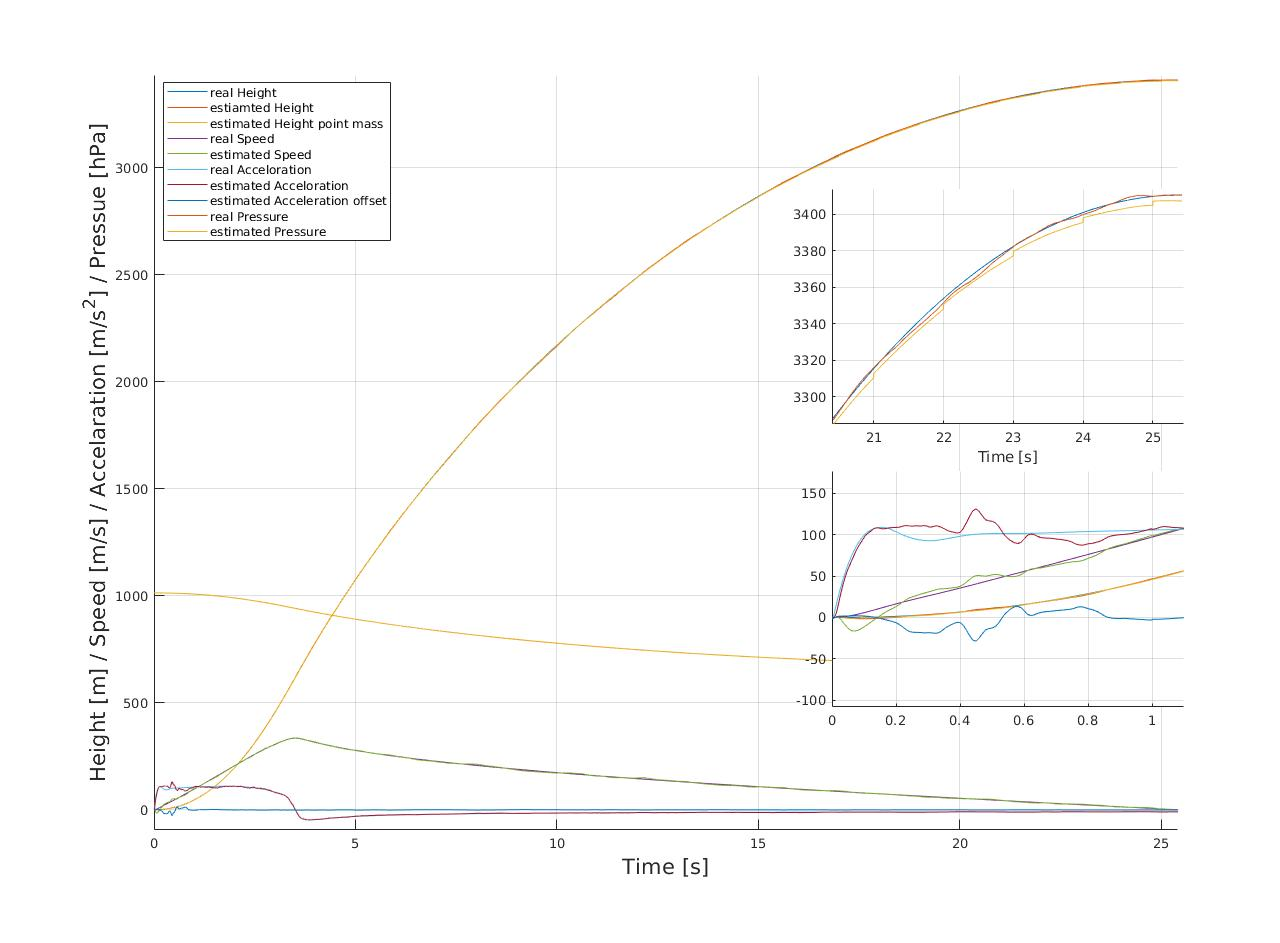
\includegraphics[width=.8\textwidth]{./Pictures/BestSystemPerformance.jpg}
 % BestSystemPerformance.jpg: 0x0 pixel, 300dpi, 0.00x0.00 cm, bb=
 \caption{Performance over time}
 \label{fig:BestSystemPerformance}
\end{figure}

Figure \ref{fig:BestSystemPerformance} shows again the performance over one whole flight.
In the plot in the lower right corner which shows the first second of the estimation it can be seen that this system has a clearly visible settling time in the acceleration and speed.
While this seems quite big at the first sight, it is well in the given requirements of one second settling time after the burnout.
On the other hand it shows that the performance increases significantly after the acceleration and speed have settled.
This increase in the accuracy of the estimation can also be seen in the table \ref{tab:ErrorBestPerformanceSystem}.

\begin{table}[h!]
\centering
\begin{tabular}{cccccc}
\hline
\multicolumn{1}{|c|}{State Variable} & \multicolumn{1}{c|}{Unit} & \multicolumn{1}{c|}{Max} & \multicolumn{1}{c|}{Min} & \multicolumn{1}{c|}{Mean} & \multicolumn{1}{c|}{Median} \\ \hline
Height                            & $m$                         & 7.39	                  & 2.01e-06                 & 1.26                    & 0.92                      \\
Speed                             & $m/s$                       & 24.87                   & 0                        & 1.61                    & 1.26                      \\
Acceleration                       & $m/s^2$   			& 41.66                   & 4.86-06                  & 1.28                    & 0.70                     \\
Acceleration Offset                & $m/s^2$   			& 41.70                   & 5.36e-06                 & 1.01                    & 0.61                     \\
Pressure		          & $hPa$   			& 0.80                    & 2.49e-06                 & 0.14                    & 0.12
\end{tabular}
\caption{Error of estimated state variables of the best found system}
\label{tab:ErrorBestPerformanceSystem}
\end{table}

While the median of the error from the estimated height shows a slight loose in the height accuracy in comparison to the system model with better system noise alone,
the accuracy of all other values has increased.
This is especially impressive in the mean of the speed and acceleration, because they have big errors at the beginning with the shown settling problem which has been shown in the plot above.
Also the height is with a median of just 0.82 meter and a maximum of 7.39 meter still most of the time in the aimed error of 2 meter maximal error.

\subsection{Robustness}
The slight loss in accuracy was traded for an increase in robustness which is seen as more important due too different uncertainties.
They are still being able to function if a sensor fails which will be covered below as well as being robust against false system modelling
and especially falsely detected temperature gradients. The impact of those errors on the found best performing system will be shown in the following sections.

\subsubsection{Without GPS}
As stated above this system should estimate the height without a significant raise in the error without the GPS measurements.
Figure \ref{fig:ErrorWitoutGPS} shows the height error of the best system model without GPS measurements.
For comparison there is also the point mass system model estimation with and without the GPS measurements plotted.

\begin{figure}[h!]
 \centering
 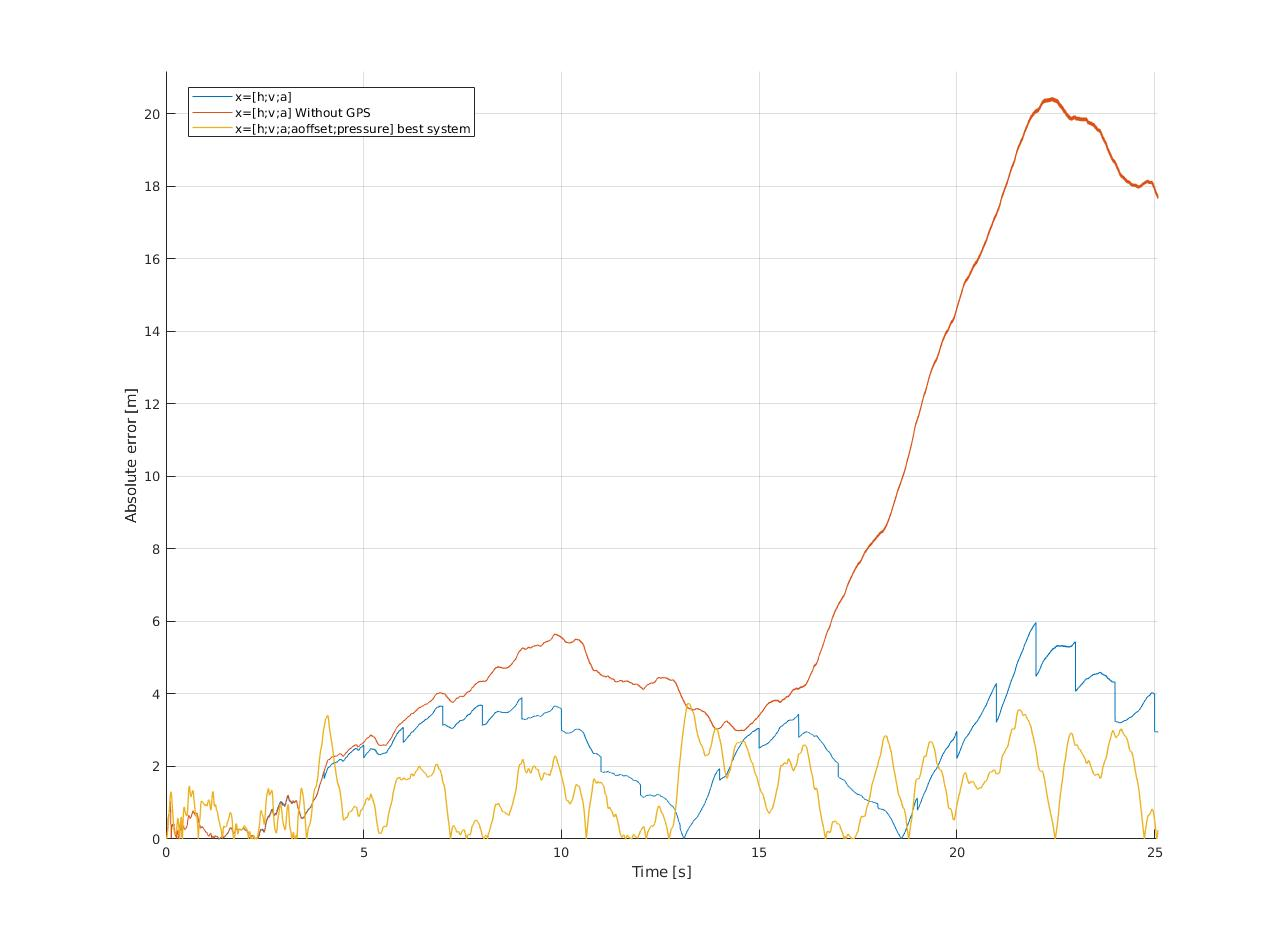
\includegraphics[width=.8\textwidth]{./Pictures/ErrorPointMassBestSystemWithoutGPS.jpg}
 % ErrorPointMassBestSystemWithoutGPS.jpg: 0x0 pixel, 300dpi, 0.00x0.00 cm, bb=
 \caption{Error of point mass system and best system with and without GPS measuements}
 \label{fig:ErrorWitoutGPS}
\end{figure}

This shows that the best found system model can estimate the height as good as the point mass system without the GPS measurements.
On the other hand the point mass system model without the GPS measurements does lose accuracy as the rocket rises higher above ground.

\subsubsection{Wrong temperature gradient}
This system model should also have some robustness against a falsely defined temperature gradient.
It has to be said that in the simulation the difference of the real and the used temperature gradient is known and the noises are adjusted properly.
This will maybe not be the case in the real flight.
Table \ref{tab:ErrorChangingTempGradWithWithoutGPS} shows the errors which the state estimation makes when the temperature gradient is wrong with and without working GPS.

\begin{table}[h!]
\centering
\begin{tabular}{ccc}
\hline
\multicolumn{1}{|c|}{Temperature gradient correctness} & \multicolumn{1}{|c|}{Mean}& \multicolumn{1}{|c|}{Median} \\ \hline
Normal with GPS 	& 1.26 		& 0.92\\
Normal without GPS	& 1.43	 	& 1.11\\
5\% off with GPS 	& 2.77	 	& 2.46\\
5\% off without GPS 	& 3.39	 	& 3.24\\
10\% off with GPS 	& 6.32	 	& 7.04\\
10\% off without GPS 	& 7.74 		& 7.61
\end{tabular}
\caption{Error of the height in meter by changing temperature gradient with and without GPS measurements}
\label{tab:ErrorChangingTempGradWithWithoutGPS}
\end{table}

First of all it can be seen that with the correct temperature gradient and no GPS measurements,
the error of the height estimation is still clearly below the two meter margin.
In addition the median of the height error does only increases by around one meter if no GPS is available.
But also the robustness of this system model can be seen, if there are no GPS measurements
and the temperature gradient is 10 percent off over the whole flight it only results in a median error of the height estimation of 7.61 meter.

\section{Sensor Outfall}
In addition to the tests for the different system model implementation
the possibility to simulate outfalls of the different sensors at start or during the flight was implemented for the last system model.
For this the corresponding measurement noise of this sensors values can be set to infinity at given time step.
The most possible way was found that a sensor fails during the burning of the motor due to the vibration.
Therefore the here discussed scenarios are all the same with the corresponding sensor failing at the third second of the flight while the motor is burning.

\subsection{GPS Outfall}
The outfall of the GPS was already discussed above which would represent a state estimation with no GPS measurements at all.
If the GPS falls out during the flight the behaviour of the state estimation should resemble the one above after the outfall.
The test have shown that this is the case.
If the GPS falls out at second three the mean of the height error rises to 1.42 meter while the median rises to 1.11 meter.
The other state variable errors rise too by a small amount but as expected the pressure estimation error stays the same.
These values show that the estimation is just slightly better than without any GPS at all.

\subsection{Barometer Outfall}
The barometer is special because if all barometers are lost,
the height which is calculated out of the state vector pressure has also to be set to failed.

\subsubsection{One Barometer fails}
The loss of one barometer does already make a significant change into the estimation.
For example the mean of the height error rises to 1.78 meter while the median also rises to 1.39 meter.
The difference between the mean and the median shows that there occur more outliers if just one barometer is active.
This can also be seen in the error of the barometer estimation which rises to 0.2 hP for the mean and 0.16 hP for the median.

\subsubsection{All Barometer fail}
More interesting is how the state estimator is performing when no barometer measurements are available at all.
As expected the error of the barometer estimation does rise onto great values which are around 12 hP for the mean and 11 hP for the median.
But on the other hand the accuracy of the height estimation does actually rise to more or less the same values as with two working barometers.
This behaviour can be explained with the still working GPS.
If both barometers fall out and therefore there is no height calculated out of the pressure, the height from the
GPS sensor gets a higher weight due to it being the only remaining measurements on the height.

\newpage
\subsection{Accelerometer Outfall}
The influence of an outfall of the accelerometer can be well visited in the plots of Figure \ref{fig:PerformanceAccOutfall}.

\begin{figure}[h!]
 \centering
 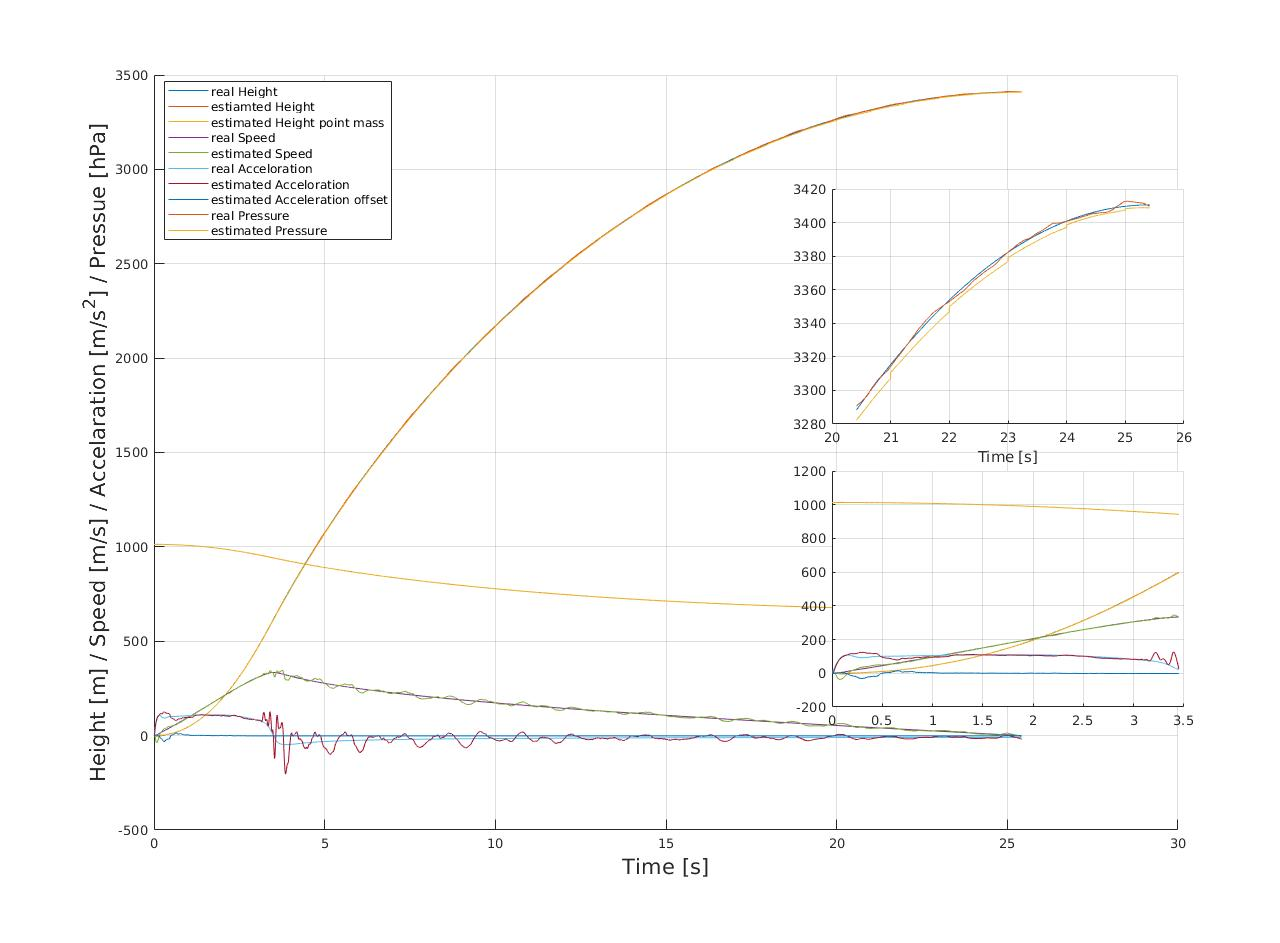
\includegraphics[width=.8\textwidth]{./Pictures/BestSystemPerformanceAccOutfall.jpg}
 % ErrorPointMassBestSystemWithoutGPS.jpg: 0x0 pixel, 300dpi, 0.00x0.00 cm, bb=
 \caption{Performance over a whole flight with failing accelerometer at second 3}
 \label{fig:PerformanceAccOutfall}
\end{figure}

It shows how the acceleration estimation starts to change in great manner after the third second.
But as it can be seen in the plot of the last five seconds the height estimation does not change in a great manner
compared to the estimation with acceleration measurements during the whole flight.
The calculated height errors do confirm this by values of 1.54 meter for the mean and 1.20 meter for the median.
The pressure estimation is not impacted as it was expected.
Also the error of the acceleration does rise by around 10 $m/s^2$ and does therefore also effect the speed estimation.

\subsection{Gyrometer Outfall}
Due to the fact that the pitch angle does not have such a great impact onto the acceleration as already stated above,
the effect onto the state estimation if the gyrometer fails is also quite small.
First of all the error which is made in the estimation of the acceleration should be examined.
Against the expectation it does rise by around 1$m/s^1$ for each the mean and also the median value.
Due to that the estimation of the height does also lose some accuracy and is with 1.39 meter for the mean
and 1.11 meter for the mean resemble the same situation as if there would be no GPS measurements.
This shows that while it is not necessary to estimate the pitch angle the measurements of the gyrometer should still be included for an optimal estimation.

\newpage
\subsection{Multiple Sensor Outfall}
A requirement which was stated is that the sensor fusion should be able to work without 2-3 sensors.
Two sensors was already discussed like if both barometer or the accelerometer
(which would also resemble the outfall of the gyrometer, since those measurements would not be included either) fails.
An additional test should therefore be what happens when three sensor fail.
For this scenario the two barometers and the GPS were chosen to fail because if they fail the observably of the point mass system is still secured.

\begin{figure}[h!]
 \centering
 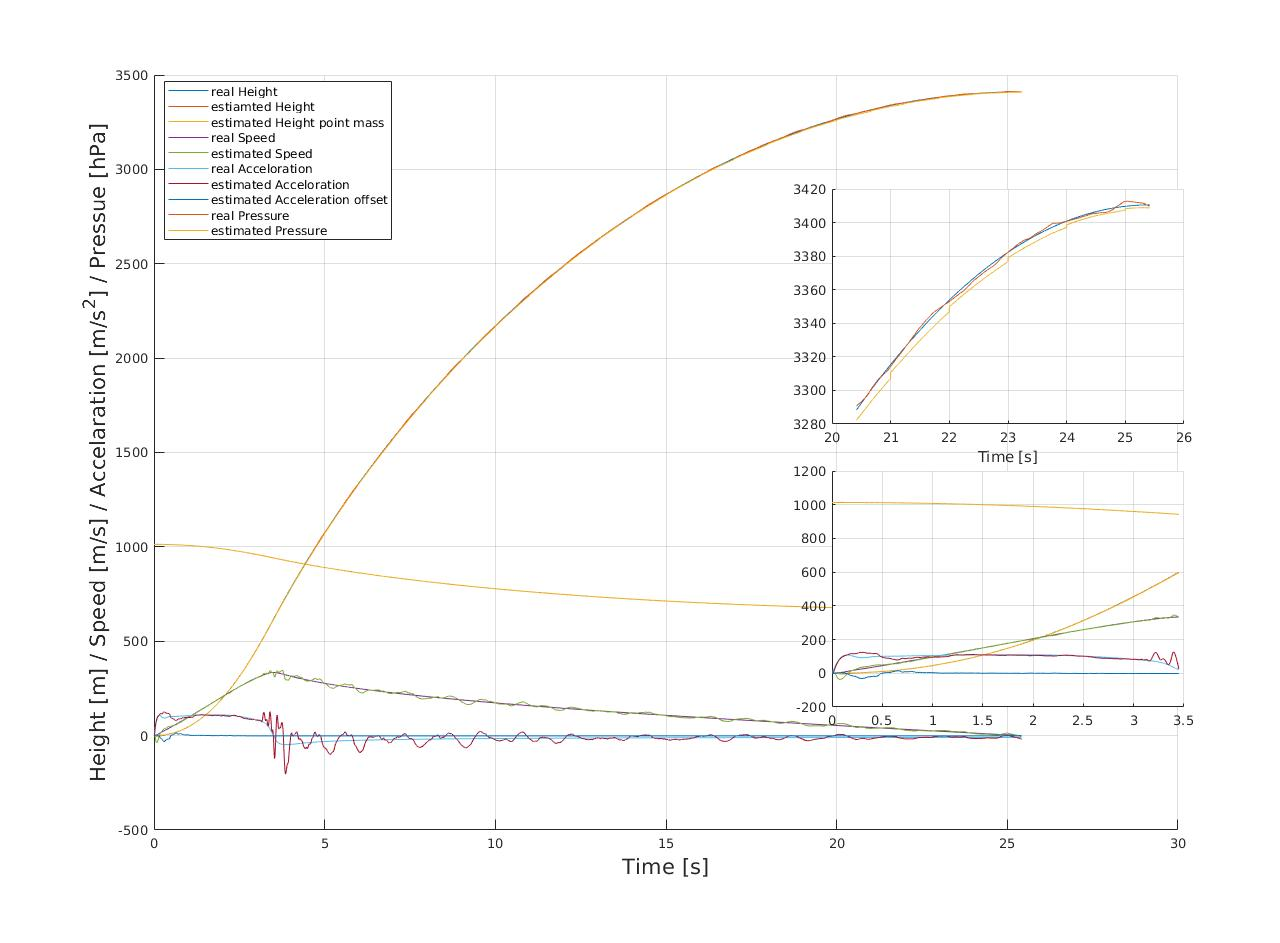
\includegraphics[width=.8\textwidth]{./Pictures/BestSystemPerformanceAccOutfall.jpg}
 % ErrorPointMassBestSystemWithoutGPS.jpg: 0x0 pixel, 300dpi, 0.00x0.00 cm, bb=
 \caption{Performance over a whole flight with both barometer and the gyrometer failed}
 \label{fig:PerformanceMOutfall}
\end{figure}

With those failed sensors the estimation does still work quite well which can be seen in the plots of the figure \ref{fig:PerformanceMOutfall}.
This is because the GPS which provides the most accurate measurements is still working.
Due to that the error of the height estimation does just rise slight amount to 1.54 meter for the mean and 0.97 meter for the median.
For comparison if the GPS sensor does also fail the height estimation does lose accuracy by a great amount and so the error rises to 63 meter for the mean and 26 meter for the median.
Also it should be said that the height error does end to 531.78 meter which is quite far off.


\chapter{Conclusion}
\label{ch:Conclusion}
\section{Derived Solution}
The solution for the stated problem which was found over this thesis can be summaryzed as follows.
The algorithm uses a discrete Kalman-filter which has dynamic noise matrices for the measurements as well as the system.
In the measurements noise matrices are the noises for the GPS and the Pressure set to infinity while no measurements from the GPS module or the Barometers are available.
The same concept is used if it is detected that a sensor is not working properly.
The state vector which describes the estimated system consist of the height, speed, acceleration, acceleration offset and the pressure.
To work in the optimal possible test flights with the used sensors have to be made and the noise matrices have to be calculated out of the measured data.
This provides an optimal trade off between robustness and accuracy and a small computational effort as possible.

\section{Comparison Solution/Requirements}
To how good the given requirements are met can be described by filling out the requirements table from the chapter \ref{ch:Introduction}



\section{Outlook}
As always there are points which could be developed further for better results which are stated here.
\subsection{Back calculation for later mesurements espacially GPS measurements}
\subsection{}
Different things which can be done differently in the future
- Exctented Kalman filter
- More better documented test flights.
- Back calculation for later mesurements espacially GPS measurements
- Slower sampling
- Calculating the pressure noise as good as possible find out how to detect how rwong the temperatur gradient is

\section{Thanks}
First of all credits have to be given to the whole ARIS team which supported this thesis with support
and great parts of a already functioning simulation which could be used to generated the trajectories.
Special thanks goes to Thomas bla and Fabian bla which provided there knowledge and the logging data from the test flights.
But also the EPFL team of the Matterhorn competition has to be thanked for the provided logging data.

\section{Reflection}
This thesis consist of theory like no one before that I have written.
Due to this, it was a quite new experience. 
This because the whole thesis consisted off concepts and there implementation in a simulation.


\bibliography{References}

\listoffigures

\listoftables

\begin{appendices}
\chapter{Shortcuts and formula table}
\section{Shortcuts}
\begin{tabbing}
 ARIS    \hspace{5cm} \= Akademische Raumfahrt Initiative Schweiz \\
 IREC 		\> Intercollegiate Rocket Engineering Competition \\
 SAC		\> Spaceport America Cup \\
 EPFL	  	\> École Polytechnique Fédérale de Lausanne \\
 GPS 		\> Global positioning system \\
 FIR filter 	\> Finite impulse response filter\\
 IIR filter 	\> Infinite impulse response filter\\
 AR model 	\> Auto Regressive model\\
 ARMA model 	\> Auto Regressive Moving Average model \\


\end{tabbing}

\section{Variables}
\begin{tabbing}
 A \hspace{5cm}	\= System matrix \\
 Ad 		\> Discrete system matrix \\
 B 		\> Input matrix \\
 Bd 		\> Discrete input matrix \\
 C 		\> Output matrix \\
 D 		\> Throughput matrix \\
 G 		\> System noise input matrix \\
 Gd 		\> Discrete system noise input matrix \\
 Q 		\> System noise matrix \\
 R 		\> Measurement noise matrix \\
 K 		\> Kalman gain matrix \\
 P 		\>  \\ % Do re read this
 P0 		\> Pressure at ground level \\
 T0 		\> Temperature at ground level \\
 Tgrad 		\> Temperature gradient for the actual weather condition \\
 M 		\> Molar mass of Earth's air: 0.0289644 kg/mol\\
 g 		\> Gravitational acceleration: 9.80665 m/$s^2$\\
 R 		\> Universal gas constant: 8.3144598 J/mol/K\\

\end{tabbing}


\end{appendices}



\end{document}
